\documentclass{book}
\usepackage[english]{babel}
%\usepackage{bookman}
%\usepackage{kmath,kerkis}
\usepackage{mathpazo}
\usepackage[T1]{fontenc}
\usepackage[utf8]{inputenc}

\usepackage{graphicx,tikz,wrapfig,hyperref,fancybox,cite,caption,subcaption,color}
\usepackage{amsmath,amssymb,amsthm,gnuplottex}

\definecolor{darkred}{rgb}{0.5,0,0}
\definecolor{darkgreen}{rgb}{0,0.5,0}
\definecolor{darkblue}{rgb}{0,0,0.5}

\hypersetup{colorlinks,
linkcolor=darkblue,
filecolor=darkgreen,
urlcolor=darkred,
citecolor=darkblue}

%%%%%%%%%%%%%%%%% stuff for including svg images %%%%%%%%%%%%%
\newcommand{\executeiffilenewer}[3]{%
 \ifnum\pdfstrcmp{\pdffilemoddate{#1}}%
 {\pdffilemoddate{#2}}>0%
 {\immediate\write18{#3}}\fi%
}

\newcommand{\includesvg}[1]{%
 \executeiffilenewer{#1.svg}{#1.pdf}%
 {inkscape -z -D --file=#1.svg %
 --export-pdf=#1.pdf --export-latex}%
 \input{#1.pdf_tex}%
}


\renewcommand{\(}{\begin{columns}}
\renewcommand{\)}{\end{columns}}
\newcommand{\<}[1]{\begin{column}{#1}}
\renewcommand{\>}{\end{column}}
\newcommand{\lien}[2]{\mathcal{L}_{#1}^{#2}}
\newcommand{\lie}[1]{\mathcal{L}_{#1}}
\newcommand{\colv}[2]{\begin{pmatrix}#1\\#2\end{pmatrix}}
\newcommand{\colvt}[3]{\begin{pmatrix}#1\\#2\\#3\end{pmatrix}}
\newcommand{\bb}[1]{\textbf{#1}}
\newcommand{\mb}[1]{\mathbf{#1}}
\newcommand{\para}{\paragraph}
\newcommand{\subpara}{\subparagraph}
\newcommand{\abso}[1]{\left|#1\right|}


\newtheorem{definition}{Definition}[section]
\newtheorem{claim}{Claim}[section]
\newtheorem{theorem}{Theorem}[section]
\begin{document}
\title{Investigating Impacting Dynamical Systems}
\author{Debsankha Manik}
\maketitle

\frontmatter
\chapter{Preface}
Piecewise smooth dynamical systems are of particular interest because of their 
ubiquity and the plethora of novel behaviours they exhibit.  There are very elegant existing frameworks
for analyzing different kinds of border collision bifurcations occurring in those systems.
These include the classic work on border collision of equilibria by Feigin\cite{feigin-1970}, analysis of grazing 
bifurcations using the ZDM (\bb{Z}ero-time \bb{D}iscontinuity \bb{M}apping) formalism developed by Nordmark et al. \cite{dm-orig-nordmark} and the impact map 
approach developed by Bernardo et al. \cite[p.~10]{bernardo-book}.

Using the ZDM formalism, Banerjee and Kundu analyzed the soft impacting oscillator system
and predicted the onset of chaos immediately following the grazing of a limit 
cycle \emph{except} when the ratio of the damped natural frequency of the 
system and the forcing function frequency are in integral or half integral 
ratios.  Experiments have roughly borne out this prediction, except for the 
fact that chaos has been observed to vanish in a \emph{small neighbourhood} of 
those values predicted analytically.  Here we have used the impact map formalism to 
derive the necessary conditions for chaos to vanish and matched the results with the 
experimental results.  

It has been reported previously that the lifetimes of transients in  systems 
exhibiting grazing bifurcations follow a power law pattern as the parameter 
value approaches the grazing value.  We have observed the same characteristics 
in a simple harmonic oscillator with hard impacts. We found that the transient 
lifetimes were orders of magnitude larger than what they should have been
if the impacts did not occur.   We have attempted to explain this 
behaviour by defining a quantity which represents how likely is a system to 
undergo impacts for a set of parameter values.  

\tableofcontents

\mainmatter
\chapter{Introduction}
\section{Overview}
% Piecewise smooth dynamical systems
Theory of dynamical systems enables us to gain valuable insights into many problems.  By using the powerful 
tools it provides, in many cases we can explain how a system will behave 
when the actual equations governing its evolution are too difficult to solve 
analytically.  This approach has been proved time and again to be extremely 
useful in a diverse range of areas: fluid flows, electrical circuits, 
ecological systems etc.  

However, conventional treatments of the subject generally places the demand 
that the systems be describable in terms of \emph{smooth} functions of the 
dynamical variables. There are valid reasons for doing so.  For a system's 
stability analysis, the Jacobian plays a role of paramount importance.  But 
its existence cannot be guaranteed everywhere in the phase space for non 
smooth systems.  



\begin{figure}[!htp]
\centering
\caption{Trajectory of a bouncing ball : a piecewise smooth system}
\label{fig-bouncing_ball}
\def\svgwidth{0.4\columnwidth}
\includesvg{bounce}
\end{figure}


Unfortunately, many systems we need to deal with regularly are non smooth: 
electrical circuits involving switches, systems exhibiting sliding or 
chattering motion, impacting systems etc.  One subclass of these systems is 
called  \emph{piecewise smooth} systems. The equation governing the evolution 
of these system changes the moment  the system 
co-ordinates cross what is known as a ``switching manifold'', which is a 
surface with 
dimension lower than that of the phase space.  Between any two of those 
switches, the system evolves smoothly. For example, a ball bouncing against 
the floor under the influence of gravity constitutes such a system.  Between 
any two bounces, the height of the ball $h$ is described by $\ddot{h}=-g/m$, 
where $g$ is the acceleration due to gravity and $m$ is the mass of the ball.  
The solution to the equation is a parabola, as depicted in Fig 
\ref{fig-bouncing_ball}, which is of course a smooth function.  But at the 
instance of the bounce, the velocity of the ball changes changes in a 
non-smooth manner.  Despite the simplicity of the system, it shows rich 
dynamical behaviour for certain parameter values\cite{2010arXiv1002.2448O}.  

% Examples

\section{Classification of piecewise smooth systems}
\subsection{Piecewise smooth maps}

\begin{definition}
A map  described by a \emph{finite} set of \emph{smooth} maps:

\begin{equation}
\label{eq-pwmap}
x\mapsto F_i(x,\mu)~~\forall x\in S_i
\end{equation}

is called a piecewise smooth map if:

\begin{enumerate}
\item 
\begin{eqnarray*}
S_i&\in& \mathbf{X}\hspace{2em} \forall i\\
\cup_i S_i&=&\mathbf{X}\\
S_i\cap S_j&=&\emptyset, \hspace{2em} i\ne j
\end{eqnarray*}
($X$ being the phase space of the system)
\item Each of the functions $F_i$ is smooth in both the state $x$ and the parameter 
$\mu$ throughout $S_i$.  
\end{enumerate}
\end{definition}
\para{Example: Tent map}
\begin{equation}
\label{eq-tent}
x_{n+1}=f_\mu(x_n)=\begin{cases} \mu x_n & \mathrm{for}~~ x_n < \frac{1}{2} \\ \\ \mu (1-x_n) & \mathrm{for}~~ \frac{1}{2} \le x_n \end{cases}
\end{equation}

\begin{figure}[!htp]
\caption{Tent map}
\begin{center}
\begin{gnuplot}[terminal=epslatex,terminaloptions=color solid linewidth 3,scale=0.7]
mu=0.4
unset ytics
set ytics add ('$\frac{\mu}{2}$' mu/2)
unset xtics
set arrow 1 
set xtics 0, 0.5, 1
f(x)=x<0.5?mu*x:mu*(1-x)
set samples 1000
set arrow from 0.5, graph 0 to 0.5, graph 1 nohead ls 3 lw 0.5
p [0:1][:mu/1.4]  f(x) 
\end{gnuplot}
\end{center}
\end{figure}




Now we will define a few quantities to be used extensively in the next 
sections.  

\begin{definition}
\label{def-switching_manifold}
The intersection $\Sigma_{ij}$ between the closures (i.e. the set and its limit points) of 
any pair of $S_i$'s are called the \bb{switching manifolds} of the system:\[
\Sigma_{ij}:=\bar{S_i}\cup\bar{S_j}
\]
\end{definition}
\para{Example:}
In case of the Tent map \eqref{eq-tent}, there is one switching manifold 
consisting of a single point:
$\Sigma_{12}=\left\{1/2\right\}$.  

\begin{definition}
\label{def-sing_order}
For a point $x_0\in\sigma_{ij}$, the leading order term in the power series 
expansion of $F_i(x)-F_j(x)$ about $x_0$ is called the \bb{order of singularity} of the 
map at the point $x_0$.  
\end{definition}
\para{Example:}
In case of tent map, 
\begin{align}
F_2(x)-F_1(x)&=2\mu x-\mu\\
&=0+2\mu(x-\frac{1}{2})
\end{align}
Therefore the order of singularity is $1$. \\


It is obvious that if the map has a \emph{discontinuity} at a point, the order 
of singularity at that point will be $0$. \\ 


We will later see that piecewise smooth maps arise naturally as a result of 
taking Poincaré sections of \emph{piecewise smooth flows} (Something we will 
define right now).

\subsection{Piecewise smooth flows}
Piecewise smooth flows are defined by extending the concept of piecewise smooth maps to 
continuous time systems:
\begin{definition}
A flow  described by a \emph{finite} set of ODE's:

\begin{equation}
\label{eq-pwflow}
\dot{x}=F_i(x,\mu)\hspace{2em}  \forall x\in S_i
\end{equation}

is called a piecewise smooth flow if:

\begin{enumerate}
\item 
\begin{eqnarray*}
S_i&\in& \mathbf{X}\hspace{2em} \forall i\\
\cup_i S_i&=&\mathbf{X}\\
S_i\cap S_j&=&\emptyset, \hspace{2em} i\ne j
\end{eqnarray*}

\item Each of the vector fields $F_i$ is smooth in both the state $x$ and the parameter 
$\mu$ throughout $S_i$.  

\item Each of the vector fields $F_i$  admits a solution $\varphi_i(x)$:
\begin{equation}
\label{eq-def_phi}
\dot{\varphi_i}(x,t)|_{t=0}=F_i(x)~~\forall x\in S_i
\end{equation}

that is smooth in both the state $x$ and the parameter 
$\mu$ throughout $S_i$.  
\end{enumerate}
\end{definition}

\para{Example: Oscillator with soft impacts\\}
\begin{figure}[!hbp]
\caption{Impact oscillator}
\begin{center}
\def\svgwidth{0.5\columnwidth}
\includesvg{osc-pw}
\end{center}
\end{figure}

Consider a simple harmonic oscillator driven by a driving force $G(t)$ which 
hits against another spring attached to the wall at a distance $\sigma$ from 
its equilibrium position. The equation of motion is given by:

\begin{equation}
\label{eq-soft_impact}
m\ddot{x}=
\begin{cases} 
-\gamma \dot{x}-k_1x+G(t)&\mathrm{for}~~x<\sigma
\\ \\ 
-\gamma \dot{x}-k_1x-k_2(x-\sigma)+G(t)&\mathrm{for}~~x\geq\sigma 
\end{cases}
\end{equation}

%Switching manifolds of piecewise smooth flows are defined identically to those 
%of piecewise smooth maps \eqref{def-switching_manifold}, while order of 
%singularities are defined slightly differently:\\
%
%\begin{definition}
%For a point $x_0\in\Sigma_{ij}$, the first non zero partial derivative of 
%$\varphi_i(x_0,t)-\varphi_j(x_0,t)$ with respect to $t$ at $t=0$ is called the \bb{order of 
%singularity} of the 
%flow at the point $x_0$.  
%\end{definition}

\subsection{Piecewise smooth hybrid systems}
\begin{definition}
A system described by a set of ODE's and a set of \bb{reset maps}:
\begin{align}
\label{def-hybrid}
\dot{x}&=F_i(x,\mu),~~\forall x\in S_i\\
x&\mapsto R_{ij}(x,\mu),~~\forall x\in\Sigma_{ij}=\bar{S_i}\cup\bar{S_j}
\end{align}

is called a piecewise smooth hybrid system if all the $R_i$'s, $F_i$'s as well 
as the associated flows $\varphi_i$'s are smooth in both $x$ and the parameter 
$\mu$ in the appropriate regimes.  
\end{definition}

\para{Example: Oscillator with hard impacts\\}

\begin{figure}[!hbp]
\caption{Hard impacting oscillator}
\label{fig-himp}
\begin{center}
\def\svgwidth{0.5\columnwidth}
\includesvg{hardcol}
\end{center}
\end{figure}

Consider a driven simple harmonic oscillator with a hard wall at a distance 
$\sigma$ from its equilibrium position, as depicted in Fig \ref{fig-himp}.   The equation of motion is:
\begin{align}
\label{eq-hard_impact}
m\ddot{x}&=-\gamma \dot{x}-k_1x+G(t)&\mathrm{for}~~x<\sigma\\
(x,v)&\mapsto (x,-rv)&\mathrm{for}~~x=\sigma
\end{align}
Where $r$ is the coefficient of restitution, which is $1$ for perfectly 
elastic collisions.  

% Behaviours specific to it: border collision

\section{Bifurcations in piecewise smooth systems}
Piecewise smooth dynamical systems, quite naturally, can show all the usual 
types of dynamical behaviour shown by smooth dynamical systems : period 
doubling\cite[p.~166-170]{hilborn-chaos} bifurcations, 
saddle-node\cite[p.~109]{hilborn-chaos} bifurcations etc.  \\

However,  piecewise smooth systems exhibit a plethora of interesting behaviours
which involve the sudden change in the system dynamics at the switching 
manifolds and hence, which are not possible in smooth systems. An extensive mathematical 
framework to study these behaviours was first published in the Russian 
literature as early as the seventies of the last century by Mark Feigin\cite{feigin-1970}.
Then these types of behaviours were named \emph{C-bifurcations}.  Now they also go by 
the name of \emph{border collision bifurcations}. We will briefly review a few 
of these novel  behaviours now.   



\begin{figure}[!htp]
\centering
\caption{A few cases of border collision bifurcations}
\def\svgwidth{0.9\columnwidth}
\includesvg{c-bifs}
\end{figure}


\subsection{Border collision of equilibria}
Consider a piecewise smooth map:

\begin{equation}
\label{ex-pwflow}
   \dot{\mathbf{x}} = \left\{
     \begin{array}{lr}
       F_1(\mathbf{x}) & : H(\mathbf{x})<0\\
       F_2(\mathbf{x}) & : H(\mathbf{x})>0
     \end{array}
   \right.
\end{equation}

Where $H(x)=0$ defines the switching manifold:
\begin{align*}
S_1&=\left\{x:H(x)<0\right\}\\
S_2&=\left\{x:H(x)\geq0\right\}
\end{align*}

Suppose there exists an equilibrium point of the 
piecewise smooth system $x_1^*(\mu)$ in the region $S_1$ of the phase space:
\[
F_1(x_1^*(\mu))=0
\]


Now, as the parameter $\mu$ is changed, this equilibrium point will, in general, move in the phase 
space.  Sometimes it may happen that for parameter values $\mu>\mu_0$ this point $x_1^*(\mu)$ crosses the 
boundary and lands up in the region $S_2$.  But in that region $\dot{x}=F_1(x)$ 
is \emph{not the correct ODE in the first place}! Therefore $x_1^*(\mu)$ is no longer 
a fixed point.  We call it a \bb{virtual fixed point}  of the system and such a phenomenon is called 
``border collision of equilibrium''. This phenomenon was first studied by Marc 
Feigin in case of discrete time systems \cite{feigin-1999}(later extended by 
Bernardo et al. to continuous time systems \cite{bernardo-c-cases}) where he classified the dynamical 
behaviours that can take place when equilibria crosses the switching manifold and 
 derived the necessary conditions for each of them in
terms of the eigenvalues of the Jacobians at both sides of the switching 
manifold. We will now briefly discuss this approach.  

\subsubsection{Types of border collision of equilibria}
Consider a piecewise smooth flow described by \eqref{ex-pwflow}. Let's switch 
to a coordinate system such that the equations of motion look like:

\begin{equation}
\label{ex-pwflow_normal}
   \dot{\mathbf{x}} = \left\{
     \begin{array}{lr}
       F_1(\mathbf{x},\mu) & : x_n<0\\
       F_2(\mathbf{x},\mu) & : x_n\geq0
     \end{array}
   \right.
\end{equation}

(Where $x_n$ denotes the $n$-th component of $\mathbf{x}$.)

Suppose that for every value of the parameter $\mu$, $\exists$ two fixed 
points of the flow, one in each side of the switching manifold:
\begin{align}
\label{def-2fps}
F_1(\mb{x_1^*},\mu)=0,&~~{x_1^*}_n\leq 0\\
F_2(\mb{x_2^*},\mu)=0,&~~{x_2^*}_n\leq 0
\end{align}

We can also assume without loss of generality that the border collision takes 
place for the parameter value $\mu=0$ at the point $\mb{x}=0$:
\[
\mb{x_1^*}=\mb{x_2^*}=\mb{0}~~\text{if } \mu=0
\]


Then we can locally linearize the map:

\begin{displaymath}
   \dot{\mb{x}} = \left\{
     \begin{array}{lr}
       \mb{A_1x+B}\mu & : x_n<0\\
       \mb{A_2x+B}\mu & : x_n<0\\
     \end{array}
   \right.
\end{displaymath}

Where:\\
\[
\mb{A_i}=\left.  \frac{\partial F_1}{\partial \mb{x}}\right|_{x=0}
\]
and 
\[
\mb{B}=\left.  \frac{\partial F_1}{\partial \mu}\right|_{\mu=0}=\left.  \frac{\partial F_2}{\partial \mu}\right|_{\mu=0}
\]
(Assuming the flow to be continuous at $\mb{x}=0$).

Also, $\mb{A_1}$ and $\mb{A_2}$ can differ only in the $n-$th column (Again 
due to continuity, this time at $\mu=0$).


Now \eqref{def-2fps} becomes:
\begin{align}
A_1\bf{x}^*_1+\bf{B}\mu&=0\\
A_2\bf{x}^*_2+\bf{B}\mu&=0
\end{align}


Assuming $A_i$'s are invertible:

\begin{align}
\label{eq-formula-2fp}
\mb{x}^*_i=-\mb{A_i}^{-1}\mb{B}\mu&=-\frac{adj(\mb{A_i})}{det(\mb{A_i})}\mb{B}\mu
\end{align}
The fixed points $\mb{x^*}_i$ will be real iff
\[
x^*_{1_{n<0}}<0, x^*_{2{_n}}>0. 
\]  

Now, from \eqref{eq-formula-2fp}
\begin{equation}
\label{eq-formula2-2fp}
x^*_{1_k}=\frac{c^*_{1_k}}{det(\bf{A_1})}\mu, x^*_{2_k}=\frac{c^*_{2_k}}{det(\bf{A_2})}
\end{equation}

Where, \[
c^*_{i_k}=[-adj(\bf{A_i)B}]_k
\]

Because $A_1$ differs from $A_2$ only in $n-$th column, $c^*_{1_n}=c^*_{2_n}:=C$

Therefore we have:
\begin{equation}
\label{eq-final-form-2fps}
x^*_{1_n}=\frac{C}{det(\bf{A_1})}\mu, x^*_{2_k}=\frac{C}{det(\bf{A_2})}\mu
\end{equation}

\para{Cases:\\}
\begin{enumerate}
\item $det({\bf A_1})det({\bf A_1})<0$:  $x^*_{1_n}$ and $x^*_{2_n}$ always have 
opposite signs:  In that case, before border collision, there'd be 2 real (or virtual)
fixed points in opposite sides of the switching manifold. As the parameter is 
changed, they'd \emph{simultaneously} suffer border collision and become 
virtual (or real) fixed points.
\item $det({\bf A_1})det({\bf A_1})>0$:  $x^*_{1_n}$ and $x^*_{2_n}$ always have 
same signs: In that case, initially $\mb{x}_1^*$ (say) will be real and $\mb{x}_2^*$ 
virtual , and after border collision $\mb{x}_1^*$ will become virtual and $\mb{x}_2^*$ 
real.   
\end{enumerate}

\begin{figure}
\centering
\caption{Border collision of equilibria}
\def\svgwidth{0.9\columnwidth}
\includesvg{cases}
\end{figure}



\subsubsection{Period doubling at border collision of equilibria}
Sometimes it may happen that after a fixed point undergoes border collision, a 
period-2 orbit emerges.  This phenomenon was also studied in great detail by \cite{feigin-1999}.
Here we discuss in brief a very important necessary condition for this to 
happen.  

\begin{claim}
\label{claim-jacob-disc}
Consider a piecewise smooth map of the form \eqref{eq-pwmap}:

\begin{equation}
x_{n+1}=f(x_n,\mu)=\begin{cases} f_1(x_n,\mu) & \mathrm{for}~~ x_n < 0 \\ \\
f_2(x_n,\mu)&\mathrm{for}~~ x_n\geq 0 \end{cases}
\end{equation}

Suppose $\exists$ a fixed point of the map $x_1^*<0$ so long as  the parameter $\mu<0$.  
Suppose that when $\mu$ equals $0$, $x_1^*$ suffers border collision and 
increasing $\mu$ further, a period-doubling bifurcation occurs.  Then the Jacobian 
of the map must suffer a discontinuity at $0$, the point of border collision 
at the parameter value $\mu=0$
\end{claim}


\begin{figure}
\caption{An example of period doubling bifurcation at grazing\\(note the 
discontinuity of  the derivative at the switching manifold)}
\begin{subfigure}{\textwidth}
\caption{Before border collision: period 1}
\begin{center}
\def\svgwidth{0.7\columnwidth}
\includesvg{pw-perdoub-bef}
\end{center}
\end{subfigure}

\begin{subfigure}{\textwidth}
\caption{After border collision: period 2}
\begin{center}
\def\svgwidth{0.7\columnwidth}
\includesvg{pw-perdoub-aft}
\end{center}
\end{subfigure}
\end{figure}


\begin{proof}


Here we will consider the 1-dimensional case. A period doubling bifurcation occurs if on changing the parameter value of a system,
\begin{enumerate}
\item The fixed point of the first composition of the map either no longer 
exists or loses stability.  
\item A fixed point in the second composition of the map either gets created 
or becomes stable.  
\end{enumerate}

Suppose that after border collision, this period-2 orbit is now stable:
\begin{align*}
f_1(x_1)&=x_2,~~x_1<0\\
f_2(x_2)&=x_1
\end{align*}

For stability, the derivative of the second composition must be less than $1$ in magnitude:
\begin{align*}
\left|\frac{d}{dx}f_2(f_1(x_1))\right|&<1\\
\left|f_1'(x_1)f_2'(x_2)\right|&<1
\end{align*}

Now, immediately after border collision, $0<\mu\ll 1$, the period-2 orbit will be 
very close to the original period-1 fixed point: $-1\ll x_1<0, 0<x_2\ll 1$.  Therefore
\[
\left|f_1'(0)f_2'(0)\right|<1
\]

Now, supposing the Jacobian suffers no discontinuity, this condition can be 
satisfied only if:
\begin{equation}
\label{cond-perdouble}
\left|f_1'(0)\right|<1, \left|f_2'(0)\right|<1
\end{equation}


But if that is the case, then the fixed point of the \emph{first composition} 
of the map (which was an attractor before the border collision and since the 
map is assumed to be continuous in the parameter $\mu$, is still in a 
neighbourhood of $0$), is still an attractor.  But this contradicts the 
necessary condition for a period doubling bifurcation (i.e. the fixed point of 
the first composition must lose stability). Therefore condition 
\eqref{cond-perdouble} can only be satisfied if the Jacobian suffers a 
discontinuity at border collision.  


For a more general proof applicable for systems of any dimensionality, please 
refer to \cite{feigin-1999}.

\end{proof}

\subsection{Grazing bifurcation of limit cycles due to border collision}
The phenomenon of a limit cycle grazing the switching manifold of a system is encountered 
very frequently.  These systems have been studied extensively by Dankowicz and Nordmark\cite{dankowicz-nordmark-zdm}, Bernardo et al.\cite{bernardo-grazing-prl}, Banerjee and Kundu\cite{banerjee-kundu-soft} etc.


Consider a piecewise smooth flow as defined in \eqref{eq-pwflow}:

\begin{equation}
\dot{x}=
\begin{cases}
F_1(x)&~~H(x)\le 0\\
F_2(x)&~~H(x)> 0
\end{cases}
\end{equation}

Suppose there exists an orbit (henceforth assumed to be period-1, for sake of 
simplicity)  which grazes against the switching manifold defined by the 
equation $H(x)=0$ at a point $0$.  By construction, $H(0)=0$.  Now we'd like 
to know how initial conditions starting very close to this stable grazing 
orbit behave.  There exists a very powerful method of analyzing the stability 
of closed orbits of flows which goes like this:

\begin{enumerate}
\item Take a Poincaré section, which is basically a plane $P$ with dimensionality $1$ 
less than that of the phase space. Especially in case of systems driven by an 
external periodic force with time period $T$, this section is generally taken 
by looking at the system at $t=nT$ (the so-called \emph{stroboscopic Poincaré section}).
Suppose the closed orbit intersects this Poincaré plane at a point $x_0$. 

\item Now choose a point $x_1$ very close to $x_0$ and see where it lands  up 
on the Poincaré plane after time $T$. This will define a so-called 
\bb{Poincaré map}
\[
\Pi:P\to P
\]
\item By construction, $x_0$ is a fixed point of the map $\Pi$.  Hence it can 
be locally linearized:
\[
\Pi(x)-x_0\approx J(x_0)(x-x_0)
\]

Where $J=\frac{\partial \Pi}{\partial x}$.  
\item The eigenvalues of the Jacobian determine the stability of the grazing 
orbit.  If all the eigenvalues are $<1$ is magnitude then it is stable, 
otherwise not.  

\end{enumerate}
\begin{figure}[!htp]
\caption{Grazing orbit}
\label{fig-grazing-orbit}
\begin{center}
\def\svgwidth{0.8\columnwidth}
\includesvg{graz}
\end{center}
\end{figure}

As depicted in Fig \ref{fig-grazing-orbit}, when grazing takes place, certain 
initial conditions close to the grazing orbit give rise to non-impacting 
orbits and others give rise to impacting orbits.  \\


Let a very important fact be noted here: \emph{The Poincaré map derived from a 
piecewise smooth flow  
will be a piecewise smooth map}: the switching manifold being the collection of points 
$x^*\in P$ such that orbits starting from them grazes the switching manifold 
of the actual flow.  

As we showed in Claim \ref{claim-jacob-disc}, the Jacobian so obtained will 
have to be discontinuous across the switching manifold for a period doubling 
cascade to take place after grazing.  


In the next section we will discuss a way of obtaining the Poincaré map 
$\Pi$ for piecewise smooth flows: the ZDM method.  
% ZDM approach

\section{Literature survey}
\subsection{ZDM}
\label{prop-ZDM}
Consider the piecewise smooth flows defined by \eqref{ex-pwflow}.Suppose 
there exists a grazing orbit in the region $H(x)>0$ that grazes the switching 
manifold at the point $x=0$.  We impose the following restrictions on the 
system and the grazing orbit:

\begin{enumerate}
\item $H(0)=0$ (A necessary condition for $x=0$ to be a grazing point).
\item $\frac{dH}{dx}\neq 0$ (Ensuring $H$ varies smoothly with $x$, a property 
to be used later).
\item $\frac{d}{dt}\left.  H(\varphi_i(0,t))\right|_{t=0}=0$ (Assuming both 
the vector fields are tangential to the switching manifold).\footnote{
$\dot{\varphi}_i(x,t)|_{t=0}=F_i(x)$.  $\varphi_i(x,t)$ denotes an orbit 
satisfying the corresponding ODE starting from the initial co-ordinate 
$x$ at $t=0$.  }
\item $a_i^*:=\frac{d^2}{dt^2}\left.  H(\varphi_i(0,t))\right|_{t=0}>0$ 
(Ensuring that $H(x)$ attains a minimum value for any orbits close to $0$, 
another property to be used later.)\label{crit-minH}
\end{enumerate}


\begin{figure}[!htp]
\centering
\caption{ZDM}
\label{fig-ZDM}
\def\svgwidth{0.4\columnwidth}
\includesvg{ZDM_eval}
\end{figure}


Consider an orbit starting from a point $x_i$ which is close to a grazing 
orbit (See Fig \ref{fig-ZDM}). Suppose the orbit spends time $\delta_0$ to hit 
the switching manifold at the point $x_1$, then it evolves according to the 
second vector field $F_2$.  After time $\delta$, it reaches the point with 
minimum $H$, an occurrence guaranteed by property \ref{crit-minH}. After time 
$\delta'$ , it hits the switching manifold again at point $x_2$


The ZDM is defined as a map which maps $x_i$ to a point $x_3$ in zero time 
such the time taken to go from $x_i$ to $x_2$ equals the time \emph{it would 
have taken to go} from 
$x_3$ to $x_2$, if the motion were governed by the vector field $F_1$.   From Fig \ref{fig-ZDM}, it is evident that \[
ZDM(x_i)=\varphi_1(-\delta_0-\delta-\delta',x_2)
\] 

The advantage of the ZDM formalism is that any orbit starting from the point 
$x_i$ at time $0$ and ending at a point $x_f$ at time $t$, both in the region $H(x)>0$ and involving a single foray 
into the `other' side side of the flow can be written as:
\begin{equation}
\label{trajeq-ZDM}
x_f=\varphi_1(ZDM(x_i),t)
\end{equation}

without worrying about Flow 2. Of course, the information regarding the time  
spent  by the system according to Flow 2 is still there: it is hidden in the ZDM.  As 
we will see in the next subsection, provided the orbit is close to grazing, 
ZDM can be derived analytically.  

In particular, ZDM approach enables one to calculate the stroboscopic Poincaré 
maps for orbits shown in Fig \ref{fig-grazing-orbit}:
\begin{equation}
\label{eq-pmap-ZDM}
\Pi(x_i)=\varphi_1((ZDM(\varphi_1(x_i,\tau_0)),T-\tau_0)
\end{equation}

after which stability analysis becomes possible using the usual method of 
calculating the eigenvalues of the Jacobian of $\Pi$ at the fixed point.  

% Order of discontinuity: trace and Jacobian
\subsection{Narrow band chaos}
Impact oscillators as described in \eqref{eq-soft_impact} and 
\eqref{eq-hard_impact} have been studied extensively since the 1970's when 
Feigin \cite{feigin-1970} described their bifurcation structure.  We now know 
that they can exhibit extremely rich dynamical behaviour.  
Using the ZDM approach, Banerjee et al. \cite{banerjee-kundu-soft} investigated 
the grazing bifurcations in such systems.  They found that the Jacobian 
suffers a discontinuity at grazing (which, as we showed in 
Claim \ref{claim-jacob-disc}, is a necessary condition for period doubling 
bifurcation at grazing) \emph{unless} the damped natural frequency of the system 
is an integral multiple of half the frequency of the external driving force:
\begin{equation}
\label{cond-chaos-vanish}
n=\frac{2\omega_g}{\omega_{forcing}}\in \mathbb{N}
\end{equation}

This implies that chaos initiated by a period doubling cascade cannot take 
place at those specific $n$-values.  Now we will describe their method.  

\subsubsection{ZDM for soft impacting oscillator}
\label{subsec-ZDM}

\begin{figure}[!htb]
\caption{Oscillator with soft impact}
\label{fig-soft-impact}
\begin{center}
\def\svgwidth{0.5\columnwidth}
\includesvg{soft-prest}
\end{center}
\end{figure}

The system is depicted in Fig \ref{fig-soft-impact}. It consists of a 
mass $m$ attached to a spring with spring constant $k_1$ and a damper with 
damping coefficient $\gamma$. The mass being externally driven by a force 
$G(t)=F\cos{\omega t}$.  There is a massless strip of wood attached to a 
spring of spring constant $k_2$ at a distance $\sigma$ from the equilibrium 
position of the first spring.  The second spring is pre-stressed so that it
 is already compressed by an amount $d$.  The equations of motion are:
\begin{equation}
m\ddot{x}=
\begin{cases} 
-\gamma \dot{x}-k_1x+G(t)&\mathrm{for}~~x<\sigma
\\ \\ 
-\gamma \dot{x}-k_1x-k_2(x-\sigma+d)+G(t)&\mathrm{for}~~x\geq\sigma 
\end{cases}
\end{equation}

Since this is a non-autonomous\footnote{i.e. explicitly depending on time} 
system defined by a second order ODE, we can write in in an autonomous first 
order form by 
defining the state variable as a 3-dimensional vector:
\begin{equation}
\label{def-statevec}
\mb{x}=
\begin{pmatrix}
x\\
v\\
t
\end{pmatrix}
\end{equation}

as the equations of motion then become:
\begin{equation}
\label{eq-softimp-3d}
\dot{\mb{x}}=
\begin{pmatrix}
\dot{x}\\
\dot{v}\\
\dot{t}
\end{pmatrix}
=
\begin{cases}
F_1(\mb{x})=
\begin{pmatrix}
v\\
(-\gamma v-k_1x+G(t))/m\\
1
\end{pmatrix}&\mathrm{for}~~x<\sigma\\
F_2(\mb{x})=
\begin{pmatrix}
v\\
(-\gamma v-k_1x-k_2(x-\sigma+d)+G(t))/m\\
1
\end{pmatrix}&\mathrm{for}~~x\geq\sigma\\
\end{cases}
\end{equation}

At suitable parameter values, there will be grazing and impacting orbits as 
depicted in Fig \ref{fig-grazing-orbit}. In that case, we can analyze the system 
dynamics in terms of a Poincaré map taking the form:
\begin{align}
\label{eq-pmap-composed}
\Pi=N_2\circ ZDM\circ N_1
\end{align}

Where $N_1$ is a state transition matrix that takes a point $x_i$ on the 
Poincaré plane to the switching manifold and $N_2$ is the state transition 
matrix that takes  the result of applying the ZDM back to the Poincaré plane.  

$N_1$ and $N_2$ can be obtained from the solution of the driven SHO, which can 
be analytically solved.  So ZDM is the only tricky part. 


\begin{figure}[!htp]
\centering
\caption{Calculating the ZDM}
\label{fig-ZDM-calc}
\def\svgwidth{0.6\columnwidth}
\includesvg{ZDM_eval_2}
\end{figure}


As we can see  from Fig \ref{fig-ZDM-calc}, the calculation \footnote{Notice that since we are calculating 
the ZDM of a point \emph{on} the switching manifold, calculations are simpler than the general case depicted in Fig \ref{fig-ZDM}} 
involves deriving expressions for $\delta$ and $\delta'$ as a function of $x_1$ 
first.   

\para{Calculate $\delta$:}

\begin{align*}
x_1&=\varphi(x_5,-\delta)\\
H(x_1)&=H(\varphi(x_5,-\delta))\\
&\approx H(\varphi_2(x_5,0))+\frac{\partial}{\partial t}H(\varphi_2(t,x_5))\left.  
\right|_{t=0}(-\delta)\\
&+\frac{\partial^2}{\partial t^2}H(\varphi_2(t,x_5))\left.\right|_{t\approx0}\frac{\delta^2}{2}\\
&\approx H(x_5)+0+\frac{\partial^2}{\partial 
t^2}H(\varphi_2(t,0))\left.\right|_{t\approx0}\frac{\delta^2}{2}\\
&\approx H(x_5)+a_2^*\frac{\delta^2}{2}
\end{align*}

Let $H(x_5)=H_{min}(x_i)=-y^2:$ 
\begin{equation}
\label{eq-d}
\delta=y\sqrt{\frac{2}{a_2^*}}
\end{equation}


\para{Calculate ZDM:}
Using identical arguments, $\delta^{\prime}=y\sqrt{\frac{2}{a_2^*}}$ \\
Let $\delta+\delta^{\prime}=\delta_1$

Then:
\begin{align}
\label{final}
x_3&\approx x_2-F_1(x_2)\delta_1+\dot{F_1}(x_2)\frac{\delta_1^2}{2}-\ddot{F_1}(x_2)\frac{\delta_1^3}{6}\\
x_1&\approx x_2-F_2(x_2)\delta_1+\dot{F_2}(x_2)\frac{\delta_1^2}{2}-\ddot{F_2}(x_2)\frac{\delta_1^3}{6}
\end{align}

\begin{align}
\label{ZDM-final}
x_3&=x_1-(F_1-F_2)(x_2)\delta_1+(\dot{F_1}-\dot{F_2})(x_2)\frac{\delta_1^2}{2}-(\ddot{F_1}-\ddot{F_2})(x_2)\frac{\delta_1^3}{6}\\
&\approx x_1-(F_1-F_2)(x^*)\delta_1+\text{H.O.T.}
\end{align}

Now we go back to the definitions of $F_i$ for the impact oscillator 
\eqref{eq-softimp-3d} and notice:
\begin{align}
F_2(x)-F_1(x)
&=
\begin{pmatrix}
v\\
(-\gamma v-k_1x-k_2(x-\sigma+d)+G(t))/m\\
1
\end{pmatrix}
-
\begin{pmatrix}
v\\
(-\gamma v-k_1x+G(t))/m\\
1
\end{pmatrix}
\\
&=
\begin{pmatrix}
0\\
k_2(-x+\sigma-d)/m\\
0
\end{pmatrix}\end{align}

Here $x^*=\sigma$.  
Therefore $F_2(x^*)-F_1(x^*)=Q\colvt{0}{1}{0}$, where $Q=-k_2d/m$.  

Thus we have from \eqref{ZDM-final}:
\begin{align}
\label{eq-ZDM-soft}
ZDM(\bb{x})&=\bb{x}-(F_1-F_2)(x^*)\delta_1\\
&=\bb{x}+2Q\sqrt{\frac{-2H_{min}(x)}{a_2^*}}\colvt{0}{1}{0}
\end{align}


\para{Calculating the Jacobian of the Poincaré map}
For orbits close to grazing, the total Poincaré map would be given by 
\eqref{eq-pmap-composed}. Therefore the Jacobian $J$ of the map would be:
\begin{align}
\label{eq-jacob-composed}
{J}&={J_{N_2}}\cdot{J_{ZDM}}\cdot{J_{N_1}}
\end{align}


From \eqref{eq-ZDM-soft}, we get:
\begin{align}
\label{eq-jacob-soft}
J_{ZDM}&=
\begin{pmatrix}
1 & 0 & 0\\
\alpha & 1 & 0\\
0 & 0 & 1
\end{pmatrix}
\end{align}

Where $\alpha=-Q\sqrt{\frac{a^*}{-2H_{min}(x)}}H_{min}'(x)$\\
Here it should be noted that at grazing 
$H_{min}=\sigma-\sigma=0$.  Therefore we see that the Jacobian of the ZDM will 
have a singularity at grazing.  This singularity will be seen to be the root 
of the discontinuity in the Jacobian, which in turn, will cause the period 
doubling cascade.  

\subpara{Jacobian of  $N_i$\\}

By definition,
\begin{align}
\label{eq-Nmatrix}
N_1(\bb{x})&=e^{A\tau}\bb{x}~~\left[\text{Where }A=
\begin{pmatrix}
0 & 1 & 0\\
-k_1/m & -\gamma/m & 0\\
0 & 0 & 1
\end{pmatrix}\right]
\\
&=\frac{e^{-\gamma t/2}}{\omega_g}
\begin{pmatrix}
\omega_g\cos{\omega_g t}+\frac{\gamma}{2}\sin{\omega_g t} & \sin{\omega_g t} & 0\\
-k\sin{\omega_g t} & \omega_g\cos{\omega_g t}-\frac{\gamma}{2}\sin{\omega_g t} 
& 0\\
0 & 0 & 1
\end{pmatrix}\bb{x}
\end{align}

Where $\omega_g=\frac{\sqrt{4k-\gamma^2}}{2}$



Similarly,
\[
N_2(\mb{x})=e^{A(T-\tau)}\mb{x}
\]

Therefore 
\begin{align}
\label{eq-n1-jacob}
J_{N_1}&=e^{A\tau}
:=e^{-\gamma\tau/2}
\begin{pmatrix}
n_{11} & n_{12} & 0\\
n_{13} & n_{14} & 0\\
0 & 0 & 1
\end{pmatrix}
\end{align}
and
\begin{align}
\label{eq-n2-jacob}
J_{N_2}&=e^{A(T-\tau)}
:=e^{-\gamma(T-\tau)/2}
\begin{pmatrix}
n_{21} & n_{22} & 0\\
n_{23} & n_{24} & 0\\
0 & 0 & 1
\end{pmatrix}
\end{align}


Now we are in a position to investigate the discontinuity of the Jacobian.  We 
first note that the Jacobian of all three parts of the map, although 
$3\times 3$ in dimension, behaves like identity on the third co-ordinate, the 
time.  Hence it is essentially a $2\times 2$ determinant.  And it has been 
shown by Banerjee and Grebogi that any $2-$D map can, by means of a suitable 
co-ordinate transformation, be written in the form:
\[
M=
\begin{pmatrix}
a & b\\
c & d
\end{pmatrix}
=
\begin{pmatrix}
Tr(M) & 1\\
-det(M) & 0
\end{pmatrix}
\]


From \eqref{eq-n1-jacob} and  \eqref{eq-n2-jacob}  it can be easily shown that 
\[
det(J_{N_1})=e^{-\gamma\tau}, det(J_{N_2})=e^{-\gamma(T-\tau)}
\]

Also, from \eqref{eq-ZDM-soft}, \[
det(J_{ZDM})=1
\]

Therefore it is evident the determinant of the Poincaré map does not suffer 
any discontinuity.  

Now we will look at the trace.  

Using \eqref{eq-jacob-composed}:
\begin{align}
\label{eq-ZDM-total}
J&=e^{-\gamma T/2}
\begin{pmatrix}
n_{21} & n_{22} & 0\\
n_{23} & n_{24} & 0\\
0 & 0 & 1
\end{pmatrix}
\begin{pmatrix}
1 & 0 & 0\\
\alpha & 1 & 0\\
0 & 0 & 1
\end{pmatrix}
\begin{pmatrix}
n_{11} & n_{12} & 0\\
n_{13} & n_{14} & 0\\
0 & 0 & 1
\end{pmatrix}\\
&=e^{-\gamma T/2}
\begin{pmatrix}
n_{21} & n_{22} & 0\\
n_{23} & n_{24} & 0\\
0 & 0 & 1
\end{pmatrix}
\begin{pmatrix}
n_{11} & n_{12} & )\\
\alpha n_{11}+n_{13} & \alpha n_{12}+n_{14} & 0\\
0 & 0 & 1
\end{pmatrix}
\end{align}

Therefore
\begin{align}
\label{eq-trace-ZDM}
Tr(J)&=e^{-\gamma T/2}(n_{11}n_{21}+n_{13}n_{22}+\alpha(n_{11}n_{22}+n_{12}n_{24})+n_{12}n_{23}+n_{14}n_{24}+1)
\end{align}

Obviously, $\alpha$ is the only term that contains the singularity term in the 
form of $H_{min}^{-1/2}$.  We take a closer look at the coefficient of $\alpha$.  

From \eqref{eq-n1-jacob} and \eqref{eq-n2-jacob}:
\begin{align}
n_{11}&=\left\{\omega_g\cos{\omega_g \tau}+\frac{\gamma}{2}\sin{\omega_g \tau} \right\}/\omega_g\\
n_{22}&=\left\{\sin{\omega_g (T-\tau)} \right\}/\omega_g\\
n_{12}&=\left\{\sin{\omega_g \tau} \right\}/\omega_g\\
n_{24}&=\left\{\omega_g\cos{\omega_g (T-\tau)}-\frac{\gamma}{2}\sin{\omega_g (T-\tau)} \right\}/\omega_g
\end{align}


Therefore the term with possible discontinuity is
\begin{align}
&\alpha\frac{\sin{\omega_g T}}{\omega_g}\\
=&\alpha\frac{\sin{2\pi\frac{\omega_g}{\omega}}}{\omega_g}
\end{align}

This equation has a serious ramification: the discontinuity vanishes if 
\begin{equation}
\label{eq-cond-chaos-vanish}
\frac{2\omega_g}{\omega}\in\mathbb{N}.
\end{equation}

According to our Claim \ref{claim-jacob-disc}, when the two frequencies are at these exact ratio, 
there won't be any period doubling cascade on grazing.  
% Chaos narrow band vanishing for integer n : hole: no chaos unexplained
\subsection{Impact map}
\label{subsec-impact-map}
Consider the impact oscillator system described by \eqref{eq-hard_impact}
\begin{align}
m\ddot{x}&=-\gamma \dot{x}-k_1x+G(t)&\mathrm{for}~~x<\sigma\\
(x,v)&\mapsto (x,-rv)&\mathrm{for}~~x=\sigma
\end{align}
Where $r$ is the coefficient of restitution.  

\begin{figure}
\caption{Oscillator with hard impacts}
\begin{center}
\def\svgwidth{0.5\columnwidth}
\includesvg{hardcol}
\end{center}
\end{figure}

In such a system, quite often periodic orbits are observed which involve one 
or more impacts at the hard wall at $x=\sigma$. For simplicity, let's consider 
orbits with only one collision. Clearly, one necessary condition 
for such orbits to exist is:
\[
(\sigma,v)\phantom{.}^{nT}_{\mapsto}(\sigma,-v/r)
\]

Where $nT$ is the time period of the orbit.  This map is known as the 
\emph{impact map}. For a stable orbit, apart from this equation, the Jacobian 
should have eigenvalues with absolute values $<1$. This approach was used
in \cite[Ch.~2;~p.~20]{bernardo-book}, where they obtained the necessary conditions 
for saddle-node and period-doubling grazing bifurcations to occur in impact 
oscillators without damping.  
% Impact map.  Budd et al: hole: no damping

\subsection{Numerical computation of fixed points}
\label{subsec-num-comp}
The method of impact map works very well to solve for periodic orbits 
involving only one collision per cycle (termed $PnC1$ orbits)\footnote{In 
general, $PmCn$ orbit means period-$m$ orbits with $n$ collisions per cycle} with the hard wall.  But this method does not 
work well for parameters values for which stable orbits collide multiple times 
in a single cycle. Ma et al.\cite{ma-nraphson} devised a way to 
numerically compute any stable or unstable $PnCm$ orbit.  We explain the 
method below. 

\begin{figure}
\caption{A $P1C1$ orbit}
\label{fig-p1c1}
\begin{center}
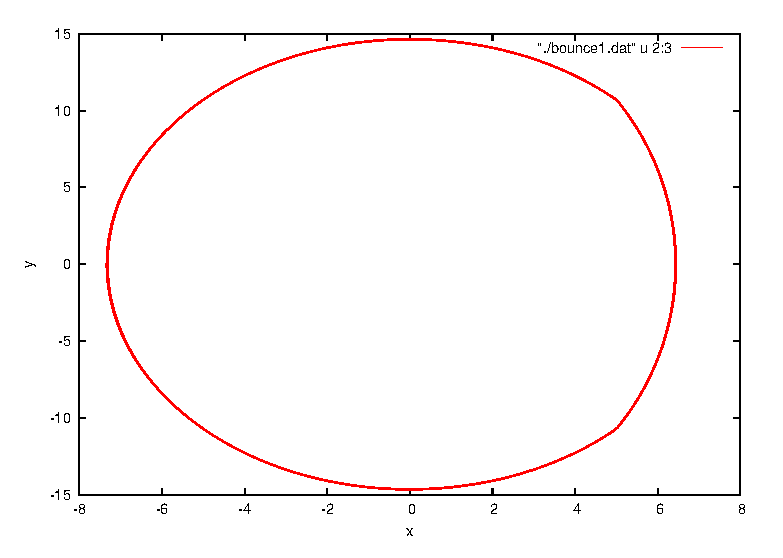
\includegraphics[width=0.5\columnwidth]{p1c1}
\end{center}
\end{figure}

For simplicity, we supposing the orbit crosses the border only once, although 
the strength of this approach is in finding more complicated orbits.  Such an 
orbit is depicted in Fig \ref{fig-p1c1}.
Then finding out the orbit boils down to finding out the solution to this set 
of equations:
\begin{align}
x_1&=\varphi_1(x_0,0,\tau_0)\\
H(x_1)&=0\\
x_2&=\varphi_2(x_1,\tau_0,\tau_1)\\
H(x_2)&=0\\
x_0&=\varphi_1(x_2,\tau_1,T-\tau_0-\tau_1)
\end{align}


This is a set of $3n+2$ equations in $3n+2$ unknowns, so this can be tackled 
with standard Newton's method of root finding:
\[
y_{n+1}=\frac{G(y_n)}{J(\bar{y}_n)}
\]

Here $y:=\left\{x_0,x_1,x_2,\tau_0,\tau_1\right\}$ is a $3n+2$ dimensional 
vector.  

Thus we can use the standard methods of stability analysis by evaluating the 
eigenvalues of the Jacobian at the fixed points.  

\subsection{Lifetime of transients}
The problem of long lived transients plagues many nonlinear systems. Despite 
the existence of a stable fixed point, trajectories starting from many initial 
conditions are found to take a lot of time to reach the fixed point.  In case 
of systems involving grazing, Grebogi et al.\cite{grebogi-transient} predicted 
that in a system where grazing occurs at parameter value $\rho=\rho_c$, 
average transient lifetimes vary as
\begin{align}
\label{form-transient-life}
\tau\propto |\rho-\rho_c|^{-\gamma}
\end{align}

Where the value $\gamma$ is called the critical transient of the system.  They 
derived an analytical expression for $\gamma$ in terms of the eigenvalues of 
the Jacobian at the fixed points of the system.  

\section{Scope of present work}
As we described in Subsection \ref{subsec-ZDM}, Banerjee et al. predicted by 
calculating the ZDM that 
chaos through on border collision route should not happen in soft impacting 
oscillators if $2\omega_g/\omega\in\mathbb{N}$.  The same analysis was found out 
to hold for hard impacting oscillators in \cite{banerjee-kundu-hard}, Experimental results were found 
to match this prediction very well. However, chaos was seen to vanish not only when $n$ were exactly 
integers, but in a small neighbourhood of each of them.  So far, no 
explanation for this has been published.  In the next chapter, we will 
take up this problem.  

% Transient lifetimes : unexplored
During our simulations on hard impacting oscillators, we observed transients 
orders of magnitude longer than what should take place in a corresponding system 
without the nonlinearity imposed by the impacts. No study on transient 
lifetimes in impacting systems had been published so far.  It needs to be 
checked if the results of 
Grebogi et al. \cite{grebogi-transient}, derived for maps,  holds true for 
continuous time impacting systems or 
not and if it does, whether a way to compute the critical exponent could be 
devised.  

\chapter{Our system}
As promised in the last chapter, we will now investigate two problems: the 
vanishing of chaos in hard impacting oscillator and the problem of long 
transients in the same system.  
\section{Description}
We briefly describe our system again.  

\begin{figure}[!hbb]
\caption{Hard impacting oscillator}
\begin{center}
\def\svgwidth{0.5\columnwidth}
\includesvg{hardcol}
\end{center}
\end{figure}



It consists of a driven simple harmonic oscillator with a hard wall at a distance 
$\sigma$ from its equilibrium position.   The equation of motion is:
\begin{align}
\label{eq-hard_impact2}
m\ddot{x}&=-\gamma \dot{x}-k_1x+F\cos{\omega t}&\mathrm{for}~~x<\sigma\\
(x,v)&\mapsto (x,-rv)&\mathrm{for}~~x=\sigma
\end{align}
Where $r$ is the coefficient of restitution, which is $1$ for perfectly 
elastic collisions.  In the rest of the thesis, we will assume all the 
collisions to be perfectly elastic unless explicitly stated otherwise.  

\subsection{Solution disregarding the boundary}
If we forget the boundary for a moment, the equation of motion is a non-homogeneous 
ODE.  As usual, its solution is a sum total of a \emph{homogeneous solution} 
and a \emph{particular solution}:
\begin{align}
\label{eq-shm-sol}
x(t)&=x_p(t)+x_h(t)\\
x_p(t)&=\frac{F/m}{\sqrt{(\omega_0^2-\omega^2)^2+\omega^2\gamma^2}}cos(\omega t+tan^{-1}\frac{\omega \gamma}{\omega^2-\omega_0^2})\\
x_h(t)&=\frac{e^{-\gamma t/2}}{\omega_g}\left\{(\omega_g\cos{\omega_gt}+\frac{\gamma}{2}\sin{\omega_gt})x(0) + (\sin{\omega_gt})v(0) \right\}\\
\omega_g&=\sqrt{\omega_0^2-\frac{\gamma^2}{4}}
\end{align}
% solution x_h and x_p

Here it should be noted that only the homogeneous solution contains the 
dependence on the initial conditions.  

\section{Approximate Poincaré map}
In this section we will make an attempt to derive an expression for a Poincaré 
map for our system assuming $PnC1$ orbits.  
Suppose the parameters of the system are set such that 
$\frac{F/m}{\sqrt{(\omega_0^2-\omega^2)^2+\omega^2\gamma^2}}=\sigma$
. This constitutes a steady state grazing orbit. Suppose we look at stroboscopic time slices such that the grazing orbit grazes 
the boundary at $t=\tau$. Now we perturb the system slightly so that the system hits the boundary with 
some non zero velocity at $t=\tau+\delta t$\\

Therefore we have:
\begin{eqnarray*}
\colv{x(0)}{v(0)}&=&\colv{x_p(0)}{v_p(0)}+\colv{x_h(0)}{v_h(0)}\\
\colv{x(\tau+\delta t)}{v(\tau+\delta t)}&=&\colv{x_p(\tau+\delta t)}{v_p(\tau+\delta t)}+\colv{x_h(\tau+\delta t)}{v_h(\tau+\delta t)}
\end{eqnarray*}
 

The instant after collision:\\
\begin{eqnarray*}
\colv{x}{v}&=&\colv{x_p(\tau+\delta t)}{-v_p(\tau+\delta t)}+\colv{x_h(\tau+\delta t)}{-v_h(\tau+\delta t)}\\
&=&\colv{x_p(\tau+\delta t)}{v_p(\tau+\delta t)}+\colv{x_h(\tau+\delta t)}{v_h(\tau+\delta t)}\\
& &+\colv{0}{-2v_h(\tau+\delta t)-2v_p(\tau+\delta t)} \\
\text{After a full time period T:}&&\\
\colv{x(T)}{v(T)}
&=&\vec{x_p}(T)+M(T-\tau-\delta t)\left\{\colv{x_h(\tau+\delta t)}{v_h(\tau+\delta t)}\right.\\
& &\left.+\colv{0}{-2v_h(\tau+\delta t)-2v_p(\tau+\delta t)}\right\}\\
&=&\vec{x_p}(T)+M(T)\vec{x_h}(0)\\&&+M(T-\tau-\delta t)\colv{0}{-2v_p(\tau+\delta t)-2v_h(\tau+\delta t)}
\end{eqnarray*}

Where 
\begin{eqnarray}
\label{def-huge-M-matrix}
M(t)=\frac{e^{-\gamma t/2}}{\omega_g}
\begin{pmatrix}
\omega_g\cos{\omega_g t}+\frac{\gamma}{2}\sin{\omega_g t} & \sin{\omega_g t}\\
-k\sin{\omega_g t} & \omega_g\cos{\omega_g t}-\frac{\gamma}{2}\sin{\omega_g t}
\end{pmatrix}
\end{eqnarray}

and
$\omega_g=\frac{\sqrt{4k-\gamma^2}}{2}$
 
Therefore we have our Poincaré map:
\begin{equation}
\label{map-poincare-hardcol}
\vec{x'}(T)=M(T)\vec{x'}(0)+M(T-\tau-\delta t)\colv{0}{-2v_p(\tau+\delta t)-2v_h(\tau+\delta t)}
\end{equation}

With the definition
\[
\vec{x'}(t)=\vec{x}(t)-\vec{x_p}(t)
\]

Now we draw attention to the fact that in the Poincaré map 
\eqref{map-poincare-hardcol} , the second term is the actual nonlinear term.  

If we can find expressions for $\delta t, v_p, v_h$ in terms of $x(0),v(0)$, 
the job will be done.  This can easily be done provided that the trajectory 
collides with the wall at very low velocity.  We provide the calculations in 
Appendix \ref{app-calc-poinc}.
 


\begin{figure}[!htp]
\begin{center}
\caption{Bifurcation digram for $n=2.235$, notice the brief region of chaos after grazing}
\label{fig-bif-int}
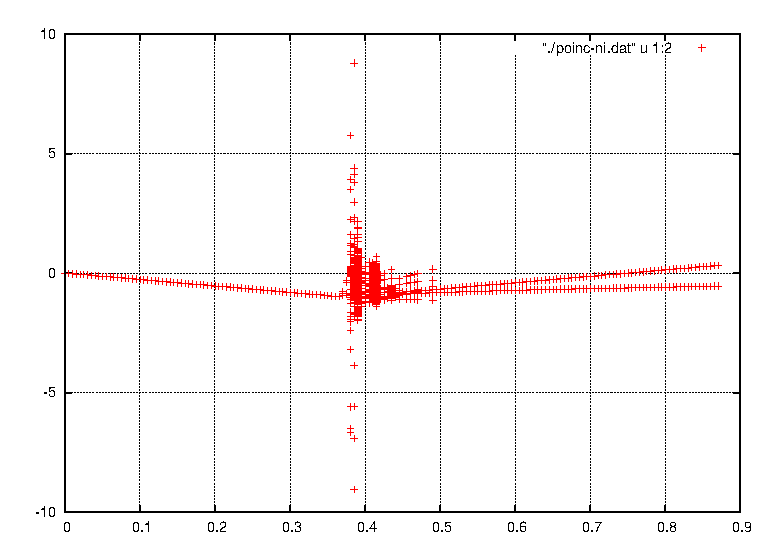
\includegraphics[width=0.6\columnwidth]{after-graz-non-int}
\end{center}
\end{figure}

\begin{figure}[!htb]
\begin{center}
\caption{Bifurcation diagram for $n=2$, notice the absence of chaos on grazing}
\label{fig-bif-nonint}
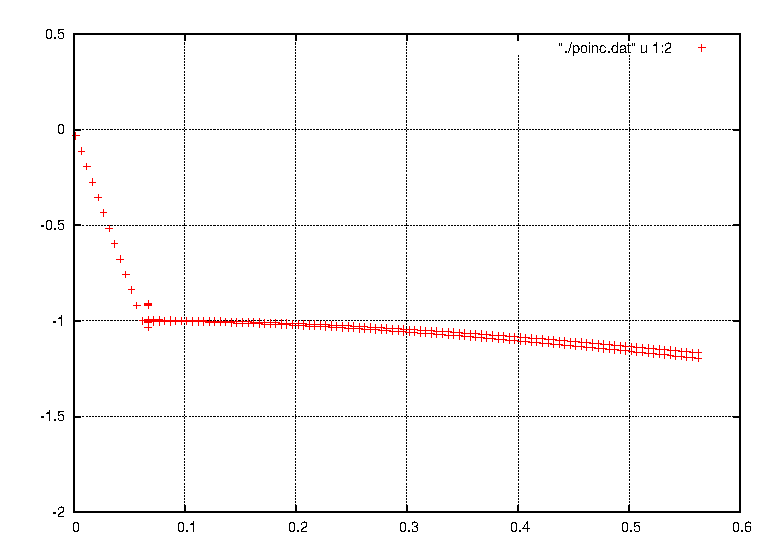
\includegraphics[width=0.6\columnwidth]{after-graz-int}
\end{center}
\end{figure}

Using this Poincaré map, we plotted the bifurcation diagrams  Fig 
\ref{fig-bif-int} and Fig \ref{fig-bif-nonint}. They clearly demonstrates the 
curious effect of making $n=\frac{2\omega_g}{\omega}$ 
an integer on grazing bifurcations. In the non-integral case, as 
\cite{banerjee-kundu-soft,banerjee-kundu-hard} predicts, there is a chaotic 
region.  But for $n=2$, no such thing happens.  Instead we see two fixed 
points immediately gaining stability. 

\section{Numerical computation of the fixed points}
We see that in case of both integral $n$ and non-integral $n$,  periodic 
orbits became stable a little bit 
after grazing.  We decided to take a look at the phase 
space trajectories. One such trajectory in case of $n=2$ is plotted in Fig \ref{fig-traj-p2c1}
\begin{figure}[!htp]
\caption{$P2C1$ orbit after grazing}
\label{fig-traj-p2c1}
\begin{center}
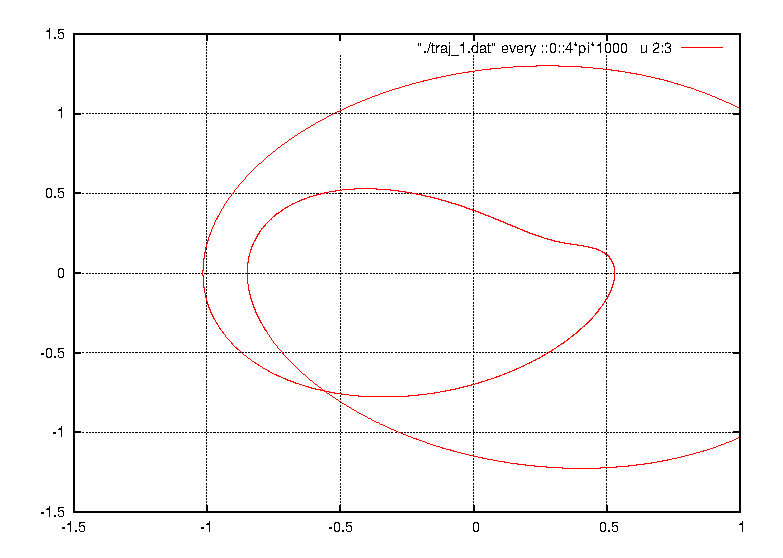
\includegraphics[width=0.9\columnwidth]{after-grazing-p1-traj}
\end{center}
\end{figure}

As we can clearly see, this is a closed orbit involving a single collision.  
The time period is $2T=2\frac{2\pi}{\omega}$.  Therefore the Newton-Raphson 
method described in Subsection \ref{subsec-num-comp} would work fine for 
stability analysis of such orbits.  

\subsection{The procedure}
We start by defining a 5-dim vector $y=(x_0,v_0,x_c,v_c,\tau)$, where $\tau$ 
is the time when a trajectory starting from $(x,v)=(x_0,v_0)$ collide with the 
hard wall and $(x,v)=(x_c,v_c)$ at that time.  

Then we get a system of equations $\mb{G}(y)=\mb{0}$ where:
\begin{align*}
G_{1,2}(y)=\vec{x_1}-\varphi(\tau,0,\vec{x_0})&=0\\
G_{3,4}(y)=\vec{x_0}-\varphi(2T,\tau,\vec{x_1})&=0\\
G_5(y)=x_1-\sigma&=0
\end{align*}

Since this is a set of 5 equations in 5 unknowns, we can solve the equation $G(y)=0$ using Newton-Raphson method:
\[
y_{n+1}=y_n+J(y)^{-1}G(y)
\]


\begin{figure}[!htp]
\caption{Modulus of  eigenvalues of the fixed points vs. the amplitude of the driving 
force for $n=2.235$}
\label{fig-eig-F-crude}
\begin{center}
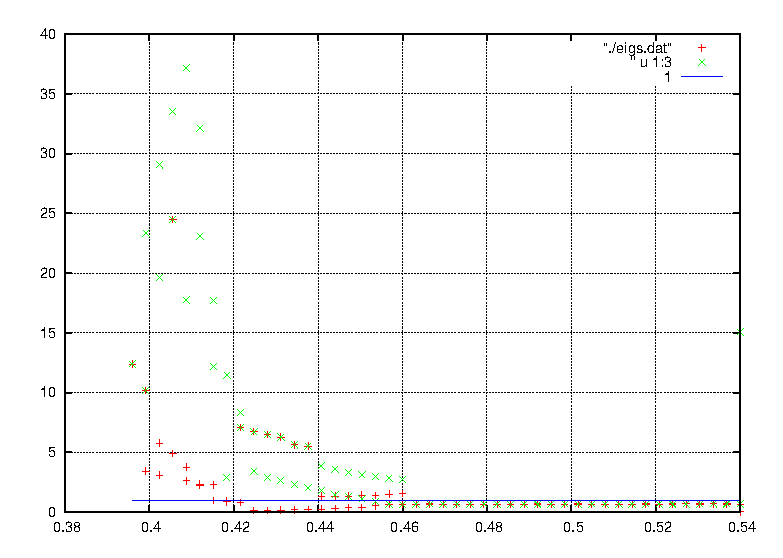
\includegraphics[width=0.7\columnwidth]{eigvals}
\end{center}
\end{figure}

\begin{figure}[!htp]
\caption{Modulus of eigenvalues of the fixed points vs. the amplitude of the driving 
force for $n=2$}
\label{fig-eig-F-n2-crude}
\begin{center}
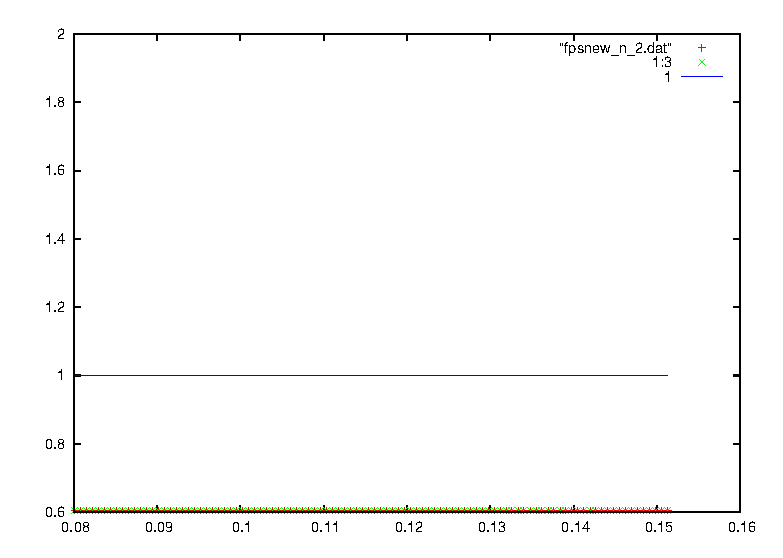
\includegraphics[width=0.7\columnwidth]{eigvals_n2}
\end{center}
\end{figure}

The solution will provide us with a $P2C1$ orbit.  It should be noted that 
this method will give \emph{stable and unstable} orbits, unlike normal 
simulations which will never give us unstable orbits.  However, in order to 
get all existing orbits, one must run the program with many initial conditions 
to ensure that the Newton-Raphson iteration scheme `finds' all the solutions.  


In Fig \ref{fig-eig-F-crude}, we plot the results of such numerical 
calculation in the case of $n=2.235$.  We can easily see that when $F$ is 
quite larger than the grazing condition (Which is $F=0.3903$, to be exact), all the 
eigenvalues are $<1$ in magnitude.  But as the $F$ value 
approaches grazing , the absolute value of one or more eigenvalues of the 
fixed point exceeds $1$.  We know from basic dynamical systems theory that 
this signifies the transition of the fixed point from attractor to repeller 
(if the magnitudes of both eigenvalues turn $>1$) or saddle (if the magnitude 
of only one  eigenvalue turn $>1$). 


However, in Fig \ref{fig-eig-F-n2-crude}, we plot the results of such numerical 
calculation in the case of $n=2$. As opposed to the previous case, no 
transition of the fixed point from an attractor to saddle/repeller takes place 
here: the eigenvalue stays put $<1$ throughout the range of parameter values. 
This again, provides a justification for the vanishing of chaos as predicted 
in \cite{banerjee-kundu-soft} . 

However, there are a few problems in the Newton-Raphson approach of stability 
analysis.  First of all, the numerically computed eigenvalues fluctuate a lot 
near grazing, possibly due to numerical errors in the Newton-Raphson iteration 
scheme.  Secondly, it does not provide us with analytical expressions for 
either the fixed points or the eigenvalues, making the task of gaining 
physical insights into the problem much more difficult.  

Therefore we decide to explore another approach for studying the same 
phenomena.  

\section{Impact map and its Jacobian}
We had described the concept of impact maps in subsection 
\ref{subsec-impact-map}. Now we will apply it in order to tackle the problem of 
stability analysis of single collision orbits in hard impacting oscillators.  


\begin{figure}[!htp]
\centering
\caption{Impact map in case of $PnC1$ orbit}
\label{fig-impmap-dia}
\def\svgwidth{0.5\columnwidth}
\includesvg{impactmap}
\end{figure}

\subsection{Derivation of the map}
Suppose the oscillator collides against the hard wall at time $\tau$ and the 
state vector immediately before collision be $\colv{x^-(\tau)}{v^-(\tau)}$.  
Just after the collision, the state vector becomes
\[
\colv{x^+(\tau)}{v^+(\tau)}=\colv{x^+(\tau)}{-v^+(\tau)}
\]

By construction, $x^-(\tau)=x^+(\tau)=\sigma$.  Then we have:

\begin{align}
\colv{x^-(\tau)}{v^-(\tau)}&=\colv{x_p(\tau)}{v_p(\tau)}+\colv{x_h(\tau)}{v_h(\tau)}\\
\colv{x^+(\tau)}{v^+(\tau)}&=\colv{x_p(\tau)}{v_p(\tau)}+\colv{x_h(\tau)}{-v_h(\tau)-2v_p(\tau)}\\
\colv{x^-(\tau+nT)}{v^-(\tau+nT)}&=\colv{x_p(\tau+nT)}{v_p(\tau+nT)}+M(nT)\colv{x_h(\tau)}{-v_h(\tau)-2v_p(\tau)}\\
&=\colv{x_p(\tau)}{v_p(\tau)}+M(nT)\colv{x_h(\tau)}{-v_h(\tau)-2v_p(\tau)}
\end{align}

Where $M(t)$ is given by \eqref{def-huge-M-matrix}.

Provided a $PmC1$ orbit exists (stable or unstable),
\[
M(mT)\colv{x_h(\tau)}{-v_h(\tau)-2v_p(\tau)}=\colv{x_h(\tau)}{v_h(\tau)}
\]

and 
\[
x_p(\tau)+x_h(\tau)=\sigma
\]
This requirement is schematically depicted in Fig \ref{fig-impmap-dia}. We recall:
\[
x_p(t)=A\footnote{$A=\frac{F/m}{\sqrt{(\omega_0^2-\omega^2)^2+\omega^2\gamma^2}}$}cos(\omega t+tan^{-1}\frac{\omega \gamma}{\omega^2-\omega_0^2})
\]

\begin{align*}
v_p(t)&=-A\omega sin(\omega t+tan^{-1}\frac{\omega \gamma}{\omega^2-\omega_0^2})\\
&=\mp A\omega \sqrt{1-\left(\frac{x_p}{A}\right)^2}\\
&=\mp A\omega \sqrt{1-\left(\frac{\sigma-x_h}{A}\right)^2}
\end{align*}

The condition for existence of a $PnC1$ orbit:
\begin{equation}
\label{impactmap-final}
M(mT)\colv{x}{-v\pm2\omega \sqrt{A^2-(\sigma-x})^2}=\colv{x}{v}
\end{equation}

The uncertainty about the $\pm$  sign is a 
direct consequence of the fact that for the same position, the velocity of the 
oscillator can have two values equal in magnitude but with opposite signs.  

Therefore now we have an expression of the impact map $M_I$ as depicted in Fig \ref{fig-impmap-dia}

\begin{align}
\label{def-mi}
M_I:\colv{x}{v}&\mapsto M(mT)\colv{x}{-v\pm2\omega \sqrt{A^2-(\sigma-x})^2}
\end{align}


\subsection{Fixed points of the map}
Therefore the fixed points of $M_I$ and the eigenvalues of the Jacobian of 
$M_I$ at those fixed points will determine whether a $PmC1$ orbit will be 
stable or not.  

Suppose
\[
M(mT)=
\begin{pmatrix}
a & b\\
c & d
\end{pmatrix}
\]

\begin{align}
\label{fp-separate}
x&=ax-bv \pm 2b\omega\sqrt{A^2-(\sigma-x)^2}\\
v&=cx-dv \pm 2d\omega\sqrt{A^2-(\sigma-x)^2}
\end{align}

$v$ can be easily eliminated:
\begin{align*}
\frac{x(1-a)+bv}{b}&=\frac{v(1+d)-cx}{d}\\
bv&=x(d-ad+bc)
\end{align*}

Substituting in \eqref{fp-separate}:
\begin{align*}
x(a-d+ad-bc-1)\pm 2b\omega\sqrt{A^2-(\sigma-x)^2}&=x\\
A^2-(\sigma-x)^2-\left\{\frac{(a-d+ad-bc-1)}{2b\omega}\right\}^2x^2&=0
\end{align*}


Let \[
\alpha=\frac{(a-d+ad-bc-1)}{2b\omega}
\]

Then:
\begin{align*}
A^2-(\sigma-x)^2&=\alpha^2x^2\\
x^2(\alpha^2+1)-2\sigma x+(\sigma^2-A^2)&=0
\end{align*}

Therefore we have the solution:
\begin{align}
\label{fp-solution}
x^*&=\frac{\sigma\pm\sqrt{\sigma^2-(\alpha^2+1)(\sigma^2-A^2)}}{\alpha^2+1}\\
v^*&=\frac{(d-ad+bc)x^*}{b}
\end{align}


One important property of  \eqref{fp-solution} is very evident:
At grazing, $A=\sigma$.  Therefore there exists a trivial solution: 
$(x^*,v^*)=(0,0)$.  This, of course, corresponds to a non-colliding orbit.  
Now, after grazing, two solutions exist simultaneously.  The question is, 
are they attractors, repellers or saddles? This is the question we will tackle 
next.  


\subsubsection{Jacobian of the map}
From \eqref{def-mi}, the Jacobian of $M_I$ can be easily calculated:
\begin{align}
\label{eq-jac-mi}
J(x,v)&=M(mT)
\begin{pmatrix}
1 & 0\\
-v\pm2\omega \frac{\sigma-x}{\sqrt{A^2-(\sigma-x})^2} & -1
\end{pmatrix}
\end{align}

\begin{figure}[!htp]
\begin{center}
\caption{Eigenvalues of fixed points Vs.  $F$ for $n=2.01,2.1,2.2$}
\label{fig-eigs-F}
\def\svgwidth{\columnwidth}
% GNUPLOT: LaTeX picture with Postscript
\begingroup
  \makeatletter
  \providecommand\color[2][]{%
    \GenericError{(gnuplot) \space\space\space\@spaces}{%
      Package color not loaded in conjunction with
      terminal option `colourtext'%
    }{See the gnuplot documentation for explanation.%
    }{Either use 'blacktext' in gnuplot or load the package
      color.sty in LaTeX.}%
    \renewcommand\color[2][]{}%
  }%
  \providecommand\includegraphics[2][]{%
    \GenericError{(gnuplot) \space\space\space\@spaces}{%
      Package graphicx or graphics not loaded%
    }{See the gnuplot documentation for explanation.%
    }{The gnuplot epslatex terminal needs graphicx.sty or graphics.sty.}%
    \renewcommand\includegraphics[2][]{}%
  }%
  \providecommand\rotatebox[2]{#2}%
  \@ifundefined{ifGPcolor}{%
    \newif\ifGPcolor
    \GPcolortrue
  }{}%
  \@ifundefined{ifGPblacktext}{%
    \newif\ifGPblacktext
    \GPblacktextfalse
  }{}%
  % define a \g@addto@macro without @ in the name:
  \let\gplgaddtomacro\g@addto@macro
  % define empty templates for all commands taking text:
  \gdef\gplbacktext{}%
  \gdef\gplfronttext{}%
  \makeatother
  \ifGPblacktext
    % no textcolor at all
    \def\colorrgb#1{}%
    \def\colorgray#1{}%
  \else
    % gray or color?
    \ifGPcolor
      \def\colorrgb#1{\color[rgb]{#1}}%
      \def\colorgray#1{\color[gray]{#1}}%
      \expandafter\def\csname LTw\endcsname{\color{white}}%
      \expandafter\def\csname LTb\endcsname{\color{black}}%
      \expandafter\def\csname LTa\endcsname{\color{black}}%
      \expandafter\def\csname LT0\endcsname{\color[rgb]{1,0,0}}%
      \expandafter\def\csname LT1\endcsname{\color[rgb]{0,1,0}}%
      \expandafter\def\csname LT2\endcsname{\color[rgb]{0,0,1}}%
      \expandafter\def\csname LT3\endcsname{\color[rgb]{1,0,1}}%
      \expandafter\def\csname LT4\endcsname{\color[rgb]{0,1,1}}%
      \expandafter\def\csname LT5\endcsname{\color[rgb]{1,1,0}}%
      \expandafter\def\csname LT6\endcsname{\color[rgb]{0,0,0}}%
      \expandafter\def\csname LT7\endcsname{\color[rgb]{1,0.3,0}}%
      \expandafter\def\csname LT8\endcsname{\color[rgb]{0.5,0.5,0.5}}%
    \else
      % gray
      \def\colorrgb#1{\color{black}}%
      \def\colorgray#1{\color[gray]{#1}}%
      \expandafter\def\csname LTw\endcsname{\color{white}}%
      \expandafter\def\csname LTb\endcsname{\color{black}}%
      \expandafter\def\csname LTa\endcsname{\color{black}}%
      \expandafter\def\csname LT0\endcsname{\color{black}}%
      \expandafter\def\csname LT1\endcsname{\color{black}}%
      \expandafter\def\csname LT2\endcsname{\color{black}}%
      \expandafter\def\csname LT3\endcsname{\color{black}}%
      \expandafter\def\csname LT4\endcsname{\color{black}}%
      \expandafter\def\csname LT5\endcsname{\color{black}}%
      \expandafter\def\csname LT6\endcsname{\color{black}}%
      \expandafter\def\csname LT7\endcsname{\color{black}}%
      \expandafter\def\csname LT8\endcsname{\color{black}}%
    \fi
  \fi
  \setlength{\unitlength}{0.0500bp}%
  \begin{picture}(7200.00,5040.00)%
    \gplgaddtomacro\gplbacktext{%
      \csname LTb\endcsname%
      \put(682,1111){\makebox(0,0)[r]{\strut{}-1}}%
      \csname LTb\endcsname%
      \put(682,1925){\makebox(0,0)[r]{\strut{} 0}}%
      \csname LTb\endcsname%
      \put(682,2740){\makebox(0,0)[r]{\strut{} 1}}%
      \csname LTb\endcsname%
      \put(682,3554){\makebox(0,0)[r]{\strut{} 2}}%
      \csname LTb\endcsname%
      \put(682,4368){\makebox(0,0)[r]{\strut{} 3}}%
      \csname LTb\endcsname%
      \put(814,484){\makebox(0,0){\strut{} 0.08}}%
      \csname LTb\endcsname%
      \put(1413,484){\makebox(0,0){\strut{} 0.09}}%
      \csname LTb\endcsname%
      \put(2012,484){\makebox(0,0){\strut{} 0.1}}%
      \csname LTb\endcsname%
      \put(2611,484){\makebox(0,0){\strut{} 0.11}}%
      \csname LTb\endcsname%
      \put(3210,484){\makebox(0,0){\strut{} 0.12}}%
      \csname LTb\endcsname%
      \put(3808,484){\makebox(0,0){\strut{} 0.13}}%
      \csname LTb\endcsname%
      \put(4407,484){\makebox(0,0){\strut{} 0.14}}%
      \csname LTb\endcsname%
      \put(5006,484){\makebox(0,0){\strut{} 0.15}}%
      \csname LTb\endcsname%
      \put(5605,484){\makebox(0,0){\strut{} 0.16}}%
      \csname LTb\endcsname%
      \put(6204,484){\makebox(0,0){\strut{} 0.17}}%
      \csname LTb\endcsname%
      \put(6803,484){\makebox(0,0){\strut{} 0.18}}%
      \put(176,2739){\rotatebox{-270}{\makebox(0,0){\strut{}Eigenvalues of Jacobian}}}%
      \put(3808,154){\makebox(0,0){\strut{}F}}%
    }%
    \gplgaddtomacro\gplfronttext{%
      \csname LTb\endcsname%
      \put(1738,4602){\makebox(0,0)[r]{\strut{}n=2.0}}%
      \csname LTb\endcsname%
      \put(1738,4382){\makebox(0,0)[r]{\strut{}n=2.0}}%
      \csname LTb\endcsname%
      \put(1738,4162){\makebox(0,0)[r]{\strut{}n=2.01}}%
      \csname LTb\endcsname%
      \put(1738,3942){\makebox(0,0)[r]{\strut{}n=2.01}}%
      \csname LTb\endcsname%
      \put(1738,3722){\makebox(0,0)[r]{\strut{}n=2.1}}%
      \csname LTb\endcsname%
      \put(1738,3502){\makebox(0,0)[r]{\strut{}n=2.1}}%
    }%
    \gplbacktext
    \put(0,0){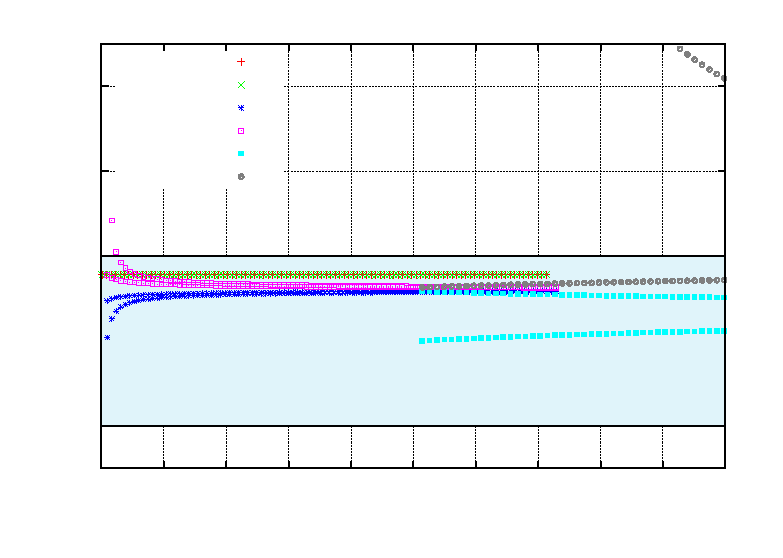
\includegraphics{./fps_various_n}}%
    \gplfronttext
  \end{picture}%
\endgroup

\end{center}
\end{figure}


In Fig \ref{fig-eigs-F}, we plot the eigenvalues of the Jacobian at the fixed 
points obtained via Formula \eqref{fp-solution} against the driving force 
amplitude for various $n$ values.  We observe that for $n=2.01$, all the 
eigenvalues at both the fixed points remain always $<1$ in magnitude, even right after grazing.  This 
means that both the fixed points are attractors.  


However, for $n=2.1$, one fixed point is an attractors throughout the whole 
range of parameter values.  However, another one is a saddle and one of its 
eigenvalues shoots up as the system approaches grazing, signifying high 
stretching of the phase space.  


In case of $n=2.2$, both of them are repellers.  Only near grazing, one of 
them become a saddle.   

\subsection{Stability analysis at grazing}
Now we are very close to determining the narrow window of disappearing chaos 
as predicted in \cite{banerjee-kundu-soft}. As we have seen in Fig 
\ref{fig-bif-nonint}, when the value of $n$ is close to a positive integer, a 
stable orbit emerges right after grazing.  Looking at the trajectories, we 
have seen that it is indeed a $P1C1$ orbit.  Therefore the window of vanishing 
chaos will be equal to the range of $n$ values where there exists an 
\emph{attracting} fixed point of the impact map $M_I$ \emph{right after grazing}.

\begin{figure}[!htp]
\begin{center}
\caption{Eigenvalues of fixed points at grazing Vs. $n$}
\label{fig-eigs-n}
\def\svgwidth{\columnwidth}
\includesvg{probing_n_2pi}
\end{center}
\end{figure}

From \eqref{fp-solution}, we can easily get the fixed points for any parameter 
values . At grazing, the expressions simplify a lot because $A=\sigma$.   
Therefore the fixed points are:

\begin{align}
\label{eq-fp-grazing}
&\begin{cases}
x_1^*&=0\\
v_1^*&=0\\
\end{cases}\\
&\begin{cases}
x_2^*&=\frac{2\sigma}{\alpha^2+1}\\
v_2^*&=\frac{(d-ad+bc)x_2^*}{b} 
\end{cases}
\end{align}

A glance at \eqref{eq-jac-mi} tells us that the Jacobian has a singular term 
at the fixed point $p_1:=(x_1^*,v_1^*)$.  This signifies infinite stretching of the 
phase space in at least one direction at that fixed point and therefore it 
cannot be an attractor.  The other one, $p_2:=(x_2^*,v_2^*)$, is therefore the one 
determining whether a $P1C1$ orbit will be stable for a certain set of 
parameter values or not.  


In Fig. \ref{fig-eigs-n} we look 
at the nature of the fixed point $p_2$ of impact map for various $n$ values. We clearly see that 
around each $n\in\mathbb{N}$, $\exists$ a neighbourhood (shaded in dark green 
in the figure), where both the eigenvalues of the Jacobian are $<1$ in 
magnitude.  The neighbourhoods are much narrower about odd $n$ values than 
they are about even $n$ values.   We also note that the neighbourhood expands 
in width as $n$ increases.  


%\begin{figure}[!htp]
%\begin{center}
%\caption{Eigenvalues of fixed points at grazing Vs. $n$}
%\label{fig-eigs-n}
%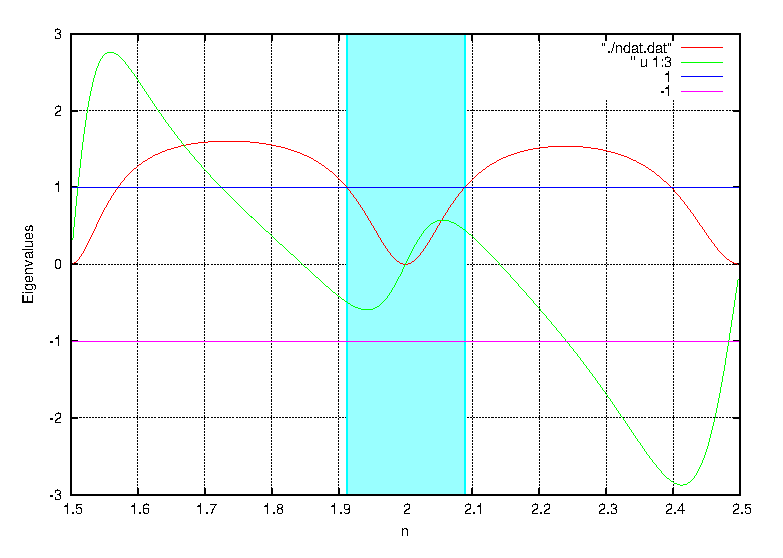
\includegraphics[width=0.7\columnwidth]{region-fp-stable-around-2}
%\end{center}
%\end{figure}




\section{Long transients}
It has previously been observed that in a system exhibiting grazing 
bifurcations, the time spent by it before settling down to its attractor 
follows a power law pattern, with a blow up at the parameter value for 
grazing.  We have observed similar results in case of  the system investigated 
in the last section, as depicted in Fig \ref{fig-tvsf} and Fig \ref{fig-tvsg}. 

\begin{figure}[!htb]
\caption{Average transient lifetime Vs.  $F$ in the hard impacting oscillator}
\label{fig-tvsf}
\begin{center}
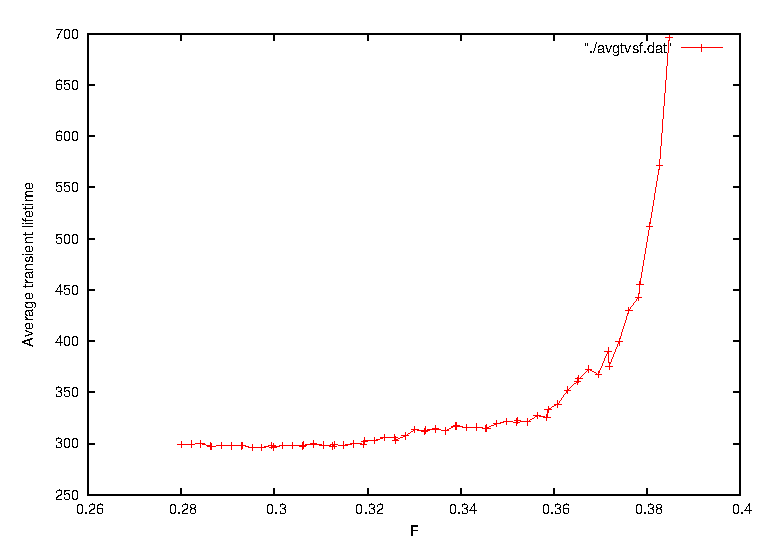
\includegraphics[width=0.7\columnwidth]{avgtauvsf-wofit}
\end{center}
\end{figure}

\begin{figure}[!htp]
\caption{Average transient lifetime Vs.  $\gamma$ in the hard impacting oscillator}
\label{fig-tvsg}
\begin{center}
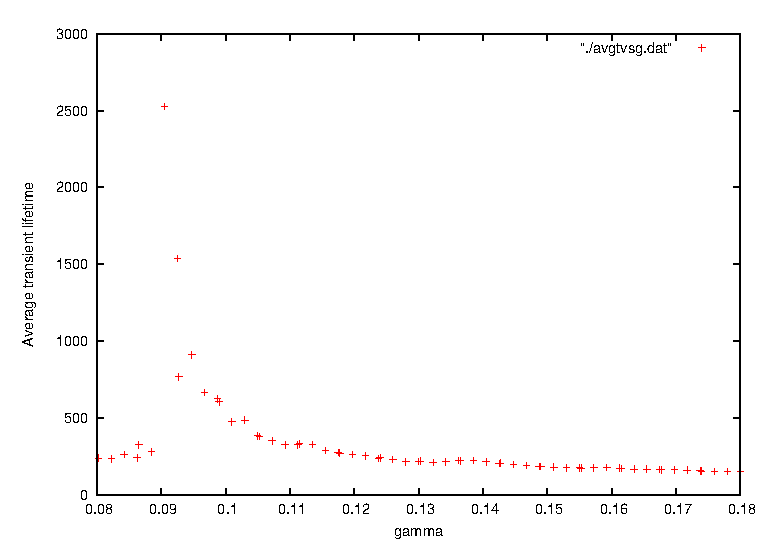
\includegraphics[width=0.7\columnwidth]{avgtauvsg-wofit}
\end{center}
\end{figure}

We point out here that these extra long lived transients are totally artefacts 
of the nonlinearity imposed by the impacts.  Because without the impacts, the 
transient solution (which we have been calling \emph{homogeneous solution} so 
far), goes as 
\begin{align}
x_h(t)&=\frac{e^{-\gamma t/2}}{\omega_g}\left\{(\omega_g\cos{\omega_gt}+\frac{\gamma}{2}\sin{\omega_gt})x_0 + (\sin{\omega_gt})v_0 \right\}
\end{align}

Therefore the transient lifetimes, if the effect of impacts is disregarded, should be \emph{inversely} proportional to 
$\gamma$ and should not depend on $F$ at all.  Therefore, in order to explain 
these long lived transients, we would need to concentrate on the impacts.  

\subsection{The no-collision area}
Consider an initial condition:
\begin{align*}
\vec{x_p}(0)&=(-A,0)\\
\vec{x_h}(0)&=(x_0,v_0)
\end{align*}

Where $A=\frac{F/m}{\sqrt{(\omega_0^2-\omega^2)^2+\omega^2\gamma^2}}$

Starting from this point, the solution till the next collision is, as per \eqref{eq-shm-sol}:

\begin{align*}
x(t)&=-A\cos{\omega t}+\frac{e^{-\gamma t/2}}{\omega_g}\left\{(\omega_g\cos{\omega_gt}+\frac{\gamma}{2}\sin{\omega_gt})x_0 + (\sin{\omega_gt})v_0 \right\}\\
&=-A\cos{\omega t}+e^{-\gamma t/2}B\cos{\left(\omega_g t+C\right)}\\
C&=-tan^{-1}\frac{\frac{\gamma}{2\omega_g}x_0+\frac{v_0}{\omega_g}}{x_0}\\
B&=\sqrt{x_0^2+\left(\frac{\gamma}{2\omega_g}x_0+\frac{v_0}{\omega_g}\right)^2}
\end{align*}

\subsubsection{Case I: $\omega\approx\omega_g$}
\begin{figure}[!htb]
\begin{center}
\caption{Plot of \eqref{eq-shm-sol} for $\omega_g\approx\omega$}
\label{fig-shm-plot}
\begin{gnuplot}[terminal=epslatex,terminaloptions=color solid linewidth 3,scale=0.7]
r=1.3
phi=1.5
m=2.2
w=3
set samples 2000
g=-0.1

set grid
se xlabel '$t$'
se ylabel '$x$'

f(x)=-cos(w*x)+r*exp(g*x/2)*cos(m*w*x/2+phi)
p [0:90] f(x) title '$-\cos{\omega x}+re^{-\gamma x/2}\cos{(m\omega x/2+\varphi)}$'
\end{gnuplot}
\end{center}
\end{figure}


In  this limit, the plot of $x$ vs.  $t$ looks almost like beats.  It is not surprising since 
\eqref{eq-shm-sol} is a superposition of two frequencies after all.   But since the amplitude associated with the 
frequency  is decaying exponentially with time, at $t\to\infty$ limit it will 
reduce to $-A\cos{\omega t}$.  

In general, the sum of two different sine waves differing both in amplitude 
and frequency cannot be further simplified.  However, an approximate envelope 
can be calculated.  

We demonstrate this in Fig \ref{fig-envelope-beats}. 

\begin{figure}[!htb]
\begin{center}
\caption{An envelope of \eqref{eq-shm-sol} for $\omega_g\approx \omega$}
\label{fig-envelope-beats}
\begin{gnuplot}[terminal=epslatex,terminaloptions=color solid linewidth 3,scale=0.7]
r=1.3
phi=1.5
m=2.2
w=3
set samples 2000
g=-0.1

set grid
se xlabel '$t$'
se ylabel '$x$'

f(x)=-cos(w*x)+r*exp(g*x/2)*cos(m*w*x/2+phi)
g(x)=(1+r*exp(g*x/2))*sin(phi/2+(m/2-1)*w*x/2)
h(x)=-(1+r*exp(g*x/2))*sin(phi/2+(m/2-1)*w*x/2)

p [0:90] f(x) title '$-\cos{\omega x}+re^{-\gamma x/2}\cos{(m\omega x/2+\varphi)}$', g(x) lt 3 title "envelope", h(x) lt 3 title ""
\end{gnuplot}
\end{center}
\end{figure}



The trajectory:
\begin{equation}
x(t)=-A\cos{\omega t}+e^{-\gamma t/2}B\cos{\left(\omega_g t+C\right)}
\end{equation}
Will have an envelope:\footnote{There are some aberrations in the first bulge 
of the envelope}
\begin{equation}
\label{eq-envelope}
E(t)=\left\{A+Be^{-\gamma t/2}\right\}\sin{\left( \frac{C+(\omega_g-\omega)t}{2} \right)}
\end{equation}


The next peak of the envelope occurs at
\begin{equation}
\label{eq-tcol}
t_c= \left\{
\begin{matrix}
\frac{\pi-C}{\omega_g-\omega}\hspace{1em} \text{if }\omega_g>\omega\\
\frac{\pi+C}{\omega-\omega_g}\hspace{1em} \text{if }\omega_g<\omega
\end{matrix}
\right.  
\end{equation}

And has height:
\begin{equation}
\label{eq-nextcolheight}
E_{m}=A+Be^{-\gamma t_c/2}
\end{equation}


\subsubsection{Case II: $\omega\gg\omega_g$}
\begin{eqnarray}
x(t)&=&-A\cos{\omega t}+e^{-\gamma t/2}B\cos{\left(\omega_g t+C\right)}\\
E(t)&=&A+e^{-\gamma t/2}B\cos{\left(\omega_g t+C\right)}
\end{eqnarray}

$E(t)$ being the upper envelope.  

\begin{figure}[!htb]
\begin{center}
\caption{An envelope of \eqref{eq-shm-sol} for $\omega_g\gg\omega$}
\begin{gnuplot}[terminal=epslatex,terminaloptions=color solid linewidth 3,scale=0.7]
r=3
phi=1.5
m=0.1
w=5
set samples 2000
g=-0.1

set grid
se xlabel '$t$'
se ylabel '$x$'

f(x)=-cos(w*x)+r*exp(g*x/2)*cos(m*w*x/2+phi)
g(x)=1+r*exp(g*x/2)*cos(m*w*x/2+phi)
h(x)=-1+r*exp(g*x/2)*cos(m*w*x/2+phi)

p [0:50] f(x) title '$-\cos{\omega x}+re^{-\gamma x/2}\cos{(m\omega x/2+\varphi)}$', g(x) lt 3 title "envelope", h(x) lt 3 title ""
\end{gnuplot}


\end{center}
\end{figure}

Therefore:
\begin{align}
t_c&=
\begin{cases}
\frac{2\pi-C}{\omega_g}&~~\text{for } C>0\\
\frac{-C}{\omega_g}&~~\text{for } C<0
\end{cases}\\
E_m&=A+Be^{-\gamma t_c/2}
\end{align}

\subsubsection{Case III: $\omega\ll\omega_g$}
\begin{eqnarray}
x(t)&=&-A\cos{\omega t}+e^{-\gamma t/2}B\cos{\left(\omega_g t+C\right)}\\
E(t)&=&-A\cos{\omega t}+e^{-\gamma t/2}B
\end{eqnarray}

\begin{figure}[!htb]
\begin{center}
\caption{An envelope of \eqref{eq-shm-sol} for $\omega_g\ll\omega$}
\begin{gnuplot}[terminal=epslatex,terminaloptions=color solid linewidth 3,scale=0.7]
r=3
phi=1.5
m=10
w=3
set samples 2000
g=-0.1

set grid
se xlabel '$t$'
se ylabel '$x$'

f(x)=-cos(w*x)+r*exp(g*x/2)*cos(m*w*x/2+phi)
g(x)=-cos(w*x)+r*exp(g*x/2)
h(x)=-cos(w*x)-r*exp(g*x/2)

p [0:8] f(x) title '$-\cos{\omega x}+re^{-\gamma x/2}\cos{(m\omega x/2+\varphi)}$', g(x) lt 3 title "envelope", h(x) lt 3 title ""
\end{gnuplot}
\end{center}
\end{figure}

Therefore:
\begin{align}
t_c&=\frac{\pi}{\omega}\\
E_m&=A+Be^{-\gamma t_c/2}
\end{align}



\subsubsection{Calculation of collision-free area}
Now we are in a position to make a quantitative measurement of how 
``collision-prone'' the system is for a certain fixed parameter value.  What 
we need to do is:

\begin{enumerate}
\item Consider a large number of initial conditions $(x_0,v_0)\in \mathbb{R}^2$.  
\item Using the envelope, predict if there will be 
any future collision or not if the system starts from that initial condition.  
\item Points for which there is no further collision should form a closed area 
in the whole space.  
\item See how this area shrinks as we approach grazing.  
\end{enumerate}

Now we will define a few quantities to be used heavily in future.  

\begin{definition}
$E_m= $ height of the next peak of the envelope.  
\end{definition}

\begin{definition}
$x_m= $ height of the next peak of the trajectory  \footnote{Except in 
some cases, $x_m=E_m$}
\end{definition}

\begin{definition}
\label{def-mu}
$\mu_{xv}=\left\{(x,v)\in\mathbb{X\times V}:x_m(x,v)<\sigma\right\}$
\end{definition}

Directly from this definition, $\mu_{xv}$ can be calculated by the Monte Carlo 
integration approach.  In Fig \ref{fig-scang} and Fig \ref{fig-scang} we 
show how $\mu_{xv}$ varies with $F$ and $\gamma$ respectively.  

\begin{figure}
\begin{center}
\caption{$\mu_{xv}$ vs.  $F$}
\label{fig-scanf}
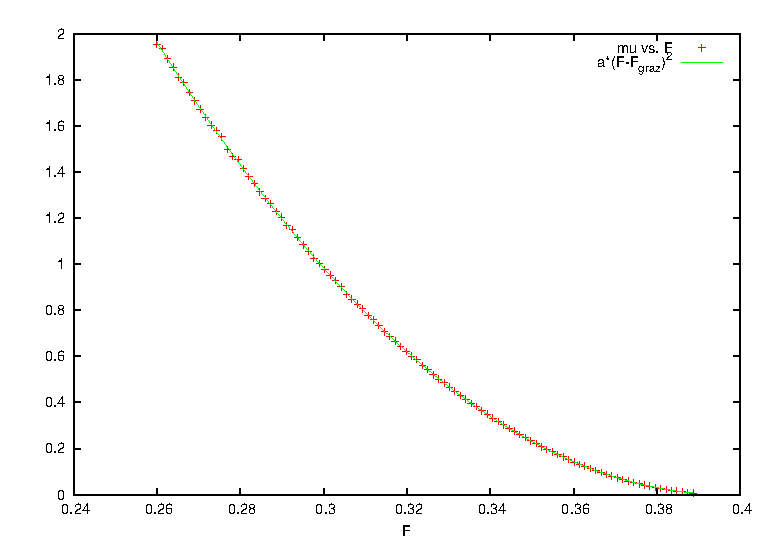
\includegraphics[width=0.8\columnwidth]{scanf}
\end{center}
\end{figure}



\begin{figure}
\begin{center}
\caption{$\mu_{xv}$ vs.  $\gamma$}
\label{fig-scang}
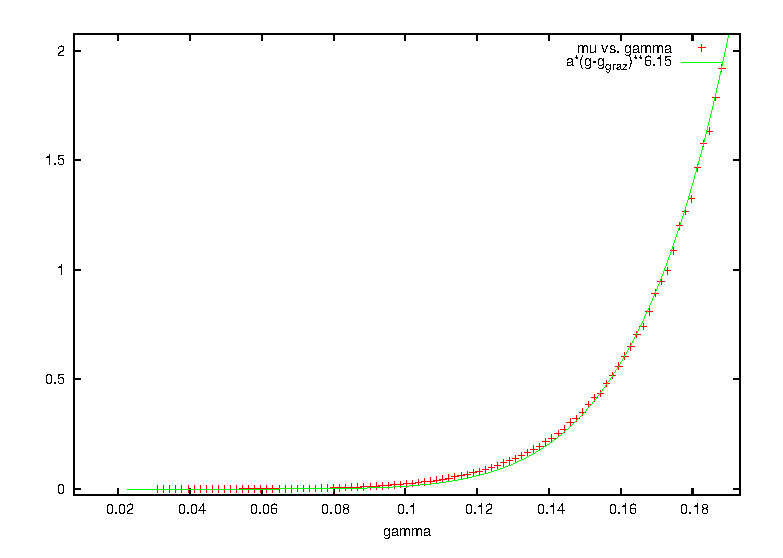
\includegraphics[width=0.8\columnwidth]{scang}
\end{center}
\end{figure}



So far, we have calculated $\mu_{xv}$ by means of a Monte Carlo integration: 
we chose $N$ initial points, evaluated the number $n$ of them that does 
not lead to collision and equated $\frac{n}{N}$ to $\mu_{xv}$.  \\

Now we'll try an analytical approach.  

\begin{align*}
\mu_{xv}&=\int_{A+B(x,v)e^{-\gamma t_c(x,v)/2}<\sigma}dxdv
\end{align*}


Now we recall \eqref{eq-tcol}
\begin{equation}
t_c= \left\{
\begin{matrix}
\frac{\pi-C}{\omega_g-\omega}\hspace{1em} \text{if }\omega_g>\omega\\
\frac{\pi+C}{\omega-\omega_g}\hspace{1em} \text{if }\omega_g<\omega
\end{matrix}
\right.  
\end{equation}


Where $C=-tan^{-1}\frac{\frac{\gamma}{2\omega_g}x_0+\frac{v_0}{\omega_g}}{x_0}$.  

Since $C$ is a rapidly varying function of both $x$ and $v$ and has range 
$\left\{-\pi/2,\pi/2\right\}$, we can replace $C\approx 0$ without too much error.  \\

Therefore 
\begin{align*}
\mu_{xv}&\sim\int_{A+B(x,v)e^{-\gamma \pi/(2|\omega_g-\omega|)}<\sigma}dxdv\\
&=\int_{B(x,v)<(\sigma-A)e^{\gamma \pi/(2|\omega_g-\omega|)}}dxdv
\end{align*}

Now we recall that 
$B=\sqrt{x_0^2+\left(\frac{\gamma}{2\omega_g}x_0+\frac{v_0}{\omega_g}\right)^2}$
.  

So our integral is now of the form:
$\int_{x^2+(ax+by)^2<\chi^2}dxdv$


\begin{align*}
&\int_{x^2+(ax+by)^2<\chi^2}dxdy\\
=&\int_{-\chi}^{\chi}dx\int_{x^2+(ax+by)^2<\chi^2} dy\\
=&\int_{-\chi}^{\chi} \frac{\sqrt{(2abx)^2-4b^2(x^2(1+a^2)-\chi^2)}}{b^2}   dx\\
=&\frac{1}{b^2}\int_{-\chi}^{\chi}2b\sqrt{\chi^2-x^2} dx\\
=&\frac{2}{b}\int_{-\chi}^{\chi}\sqrt{\chi^2-x^2} dx
\end{align*}

However, we have disregarded one very important restriction: $x<\sigma$, due to 
the hard wall.  \\

So, actually:
\begin{align}
\label{mu-analytical}
\mu_{xv}&\approx2\omega_g\int_{-\chi}^{max\{\chi,1\}} \sqrt{\chi^2-x^2}dx
\end{align}


Now it needs to be seen how good the approximations involved in deriving the 
analytical expression \eqref{mu-analytical} were.  In Fig 
\ref{fig-mu-actual-approx}, we plot values of $\mu_{xv}$ using the analytical formula and the values 
obtained by Monte Carlo integration using $100000$ points against $F$.  As we 
can see, the approximation overestimate $\mu_{xv}$ only slightly.  

\begin{figure}[!htb]
\caption{$\mu_{vx}$ vs.  $F$: comparison between the result of Monte Carlo integration
and the approximate value}
\label{fig-mu-actual-approx}
\begin{center}
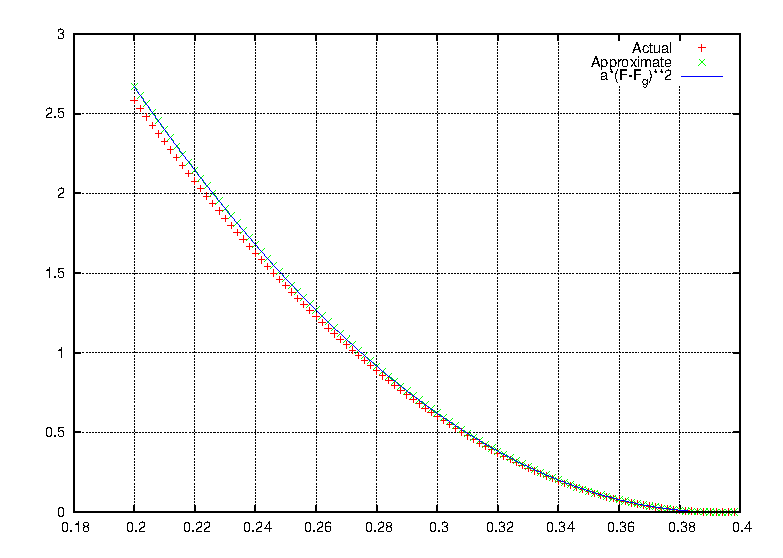
\includegraphics[width=0.75\columnwidth]{vxarea-actual-approx}
\end{center}
\end{figure}



%Recall that our calculation, both analytical and numerical, has started off 
%with an assumption.   
%Now we'll try to justify. \\
%\begin{align*}
%&\left|f(t)cos(\omega_1t)+g(t)cos(\omega_2t+C)\right|\\
%\le&\left|(f(t)+g(t))(cos(\omega_1t)+cos(\omega_2t+C))\right|\\
%=&2\left|\left\{f(t)+g(t)\right\}sin\left(\frac{(\omega_1-\omega_2)t+C}{2}\right)\right|\left|sin\left(\frac{(\omega_1+\omega_2)t+C}{2}\right)\right|
%\end{align*}
%
%Now since the last term is much more rapidly varying than the second term, we 
%replace it with its average over a full cycle without incurring too much error:
%\begin{align*}
%=&2\left|\left\{f(t)+g(t)\right\}sin\left(\frac{(\omega_1-\omega_2)t+C}{2}\right)\right|\frac{2}{\pi}\int_0^{\pi/2}cos(t)dt\\
%=&2\left|\left\{f(t)+g(t)\right\}sin\left(\frac{(\omega_1-\omega_2)t+C}{2}\right)\right|\frac{2}{\pi}
%\end{align*}
%
%
%
%\em{$\omega >> \omega_g$}
%

\subsubsection{Relationship between $\mu_{xv}$ and transient lifetime}
We see from Fig \ref{fig-scanf} and Fig \ref{fig-scang}  that $\mu_{xv}$ varies with parameters $F$ and $\gamma$ following a power law 
pattern: far from grazing, the area is large; implying plenty of chance of the 
system to go to a stable non-grazing orbit.  However, as the parameter is 
tuned towards grazing, this area sharply drops to zero; which results in 
frequent collisions with the boundary even though there exists a non-grazing 
stable orbit.  So the system takes a long time to ``find'' that elusive stable 
orbit, resulting in long transient lifetimes. 

This immediately suggests that the transient lifetime $\tau$ may be related to 
$\mu_{vx}$ according to:

\begin{align}
\label{eq-hypo-mu}
\tau\propto\frac{1}{\mu}
\end{align} 


This hypothesis is further strengthened by the fact that both $\mu_{xv}$ and 
$\tau$ have been seen to follow power law pattern.  Now it remains to check if 
the exponent for $\tau$ turns out to be $-1$ times the exponent for $\mu_{vx}$ 
or not.  

\begin{figure}
\caption{Transient lifetime vs.  $F$}
\begin{center}
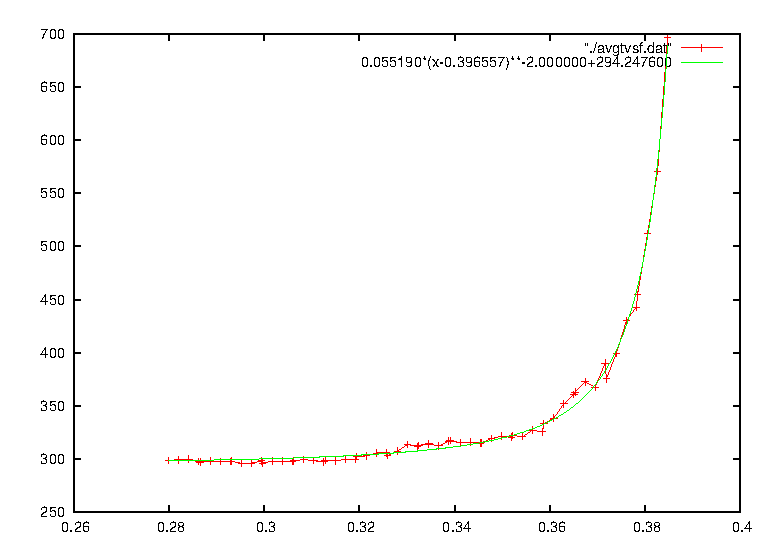
\includegraphics[width=0.8\columnwidth]{trans_life_vsf_matches}
\end{center}
\end{figure}


\begin{figure}
\caption{Transient lifetime vs.  $\gamma$}
\begin{center}
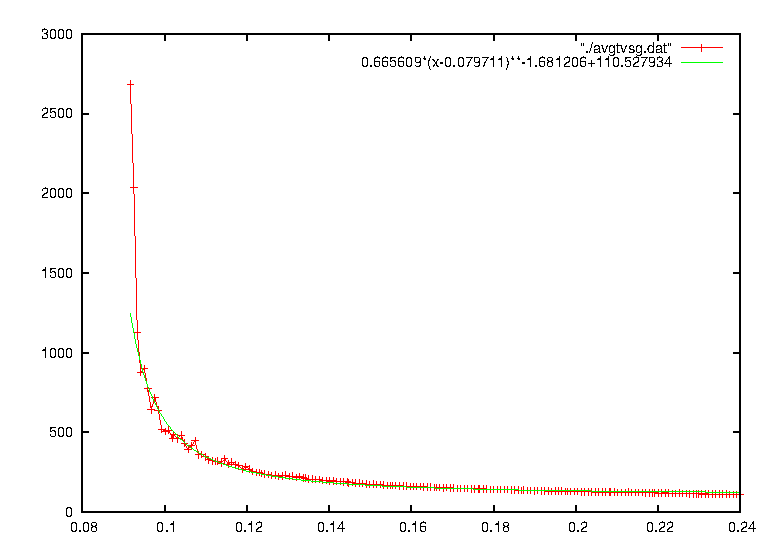
\includegraphics[width=0.8\columnwidth]{trans_life_vsg_matches_somewhat}
\end{center}
\end{figure}


\section{Conclusion}
In this thesis, we have explored two separate aspects of the impact oscillator 
system.  The first one was that of vanishing chaos when the ratio of the 
damped natural frequency of the oscillator and the frequency of the driving 
force is in the neighbourhood of certain discrete values.  So far, no 
analytical method 
for determining what these neighbourhoods are has been published. Using the 
	impact map formalism, we have done that.  This is extremely helpful
to know these neighbourhoods in actual physical systems because it will enable 
one to set system parameters in a way so that chaos is avoided.  \\

The second problem we tackled is that of extra long transient times.  This is 
a very important problem for experimenters because in every experiment one can 
afford to spend a finite amount of time for each measurement.  Extra long 
transient times can make experiments cumbersome at best and non-viable at 
worst.  We have attempted to devise a way that can explain the way these lifetimes change with any 
parameter of the system.  



\appendix
\chapter{Calculations for approximate Poincaré map}
In \eqref{map-poincare-hardcol}, there were a few unknown variables whose 
analytical expressions in the regime of low velocity collisions 
needed to be determined.  We proceed to do so now:

\label{app-calc-poinc}
Let the parameters be such that the stable orbit grazes slightly:
$x_m(\left\{parameters\right\})=\sigma+\varepsilon$.  \\

Now start from an initial condition such that $\left|x'(0)\right|=0$.  
(Exactly on the stable orbit).\\

Then we have:
\begin{align*}
x_mcos\left(\omega \tau+tan^{-1}\frac{\omega \gamma}{\omega^2-\omega_0^2}\right)&=\sigma\\
\omega \tau+tan^{-1}\frac{\omega \gamma}{\omega^2-\omega_0^2}&=cos^{-1}\left(1+\frac{\varepsilon}{\sigma}\right)^{-1}\\
&\approx2n\pi+\sqrt{\frac{2\varepsilon}{\sigma}}\\
\tau&\approx \frac{1}{\omega}\left(2\pi+\sqrt{\frac{2\varepsilon}{\sigma}}-tan^{-1}\frac{\omega \gamma}{\omega^2-\omega_0^2}\right)
\end{align*}
 

 
Now suppose $0<|x'(0)|<<1$.   
Let the time of collision $t_c=\tau+\delta t$
\begin{align*}
x_mcos\left(\omega (\tau+\delta t)+tan^{-1}\frac{\omega 
\gamma}{\omega^2-\omega_0^2}\right)+x_h(\tau+\delta t)&=\sigma\\
x_mcos\left(\left(\omega \tau+tan^{-1}\frac{\omega 
\gamma}{\omega^2-\omega_0^2}\right)+\omega \delta t\right)+x_h(\tau+\delta t)&=\sigma\\
\sigma-\omega x_m\delta t sin\left(\omega \tau+tan^{-1}\frac{\omega 
\gamma}{\omega^2-\omega_0^2}\right)+x_h(\tau+\delta t)&=\sigma\\
-\omega \delta tx_m\sqrt{1-(\sigma/x_m)^2}+x_h(\tau+\delta t)&=0\\
\frac{x_h(\tau)}{\omega\sqrt{x_m^2-\sigma^2}-v_h(\tau)}&=\delta t
\end{align*}
 

 
\begin{align*}
v_p(\tau+\delta t)&=-\omega x_m sin\left( \omega (\tau+\delta t)+tan^{-1}\frac{\omega 
\gamma}{\omega^2-\omega_0^2}\right)\\
&=-\omega x_m sin\left( 
2\pi+\sqrt{\frac{2\varepsilon}{\sigma}}-tan^{-1}\frac{\omega 
\gamma}{\omega^2-\omega_0^2}+\omega \delta t + tan^{-1}\frac{\omega 
\gamma}{\omega^2-\omega_0^2} \right)\\
&=-\omega x_m sin\left(\omega\delta t+\sqrt{\frac{2\varepsilon}{\sigma}}\right) 
\end{align*}
% plot of numerical poincare map

\bibliography{thesis}{}
\bibliographystyle{plain}
\end{document}
